\documentclass[12pt,a4paper]{article}

\usepackage[utf8]{inputenc}
\usepackage{amsmath,amssymb}
\usepackage{graphicx}
\usepackage{hyperref}
\usepackage{geometry}
\usepackage{booktabs}
\usepackage{float}
\usepackage{cite}
\usepackage{titlesec}
\usepackage{listings}
\usepackage{xcolor}
\usepackage{tikz}
\usepackage{pgfplots}
\usepackage{enumitem}
\usepackage{multicol}
\usepackage{longtable}
\usepackage{array}
\usepackage{tabularx}
\pgfplotsset{compat=1.18}
\usetikzlibrary{shapes.geometric, arrows.meta, positioning, fit, backgrounds, calc, decorations.markings, patterns, shapes.multipart, matrix, chains, scopes, shadows}

\pgfplotsset{compat=1.18}

\tikzset{
    sysblock/.style={rectangle, draw=#1, fill=#1!12, rounded corners=3pt, minimum width=2.6cm, minimum height=0.9cm, align=center, font=\sffamily\small, line width=0.6pt, drop shadow={opacity=0.1, shadow xshift=1pt, shadow yshift=-1pt}},
    sysdb/.style={cylinder, draw=#1, fill=#1!12, shape border rotate=90, aspect=0.3, minimum width=1.8cm, minimum height=1cm, align=center, font=\sffamily\small, line width=0.6pt, drop shadow={opacity=0.1, shadow xshift=1pt, shadow yshift=-1pt}},
    sysarrow/.style={-{Stealth[length=2.5mm]}, thick, gray!80, line width=0.8pt},
    sysdarrow/.style={{Stealth[length=2.5mm]}-{Stealth[length=2.5mm]}, thick, gray!80, line width=0.8pt},
    sysannot/.style={font=\sffamily\scriptsize\itshape, text=softgray, align=center},
    systier/.style={font=\sffamily\footnotesize\bfseries, text=#1!80!black, inner sep=5pt},
    syscontainer/.style={rectangle, fill=#1!5, draw=#1!20, rounded corners=8pt, dashed, line width=0.5pt, inner sep=15pt}
}

\geometry{a4paper, margin=1in}

\definecolor{edgeblue}{RGB}{59,130,246}
\definecolor{flaskgreen}{RGB}{16,185,129}
\definecolor{kafkaorange}{RGB}{245,158,11}
\definecolor{influxpurple}{RGB}{139,92,246}
\definecolor{reactcyan}{RGB}{6,182,212}
\definecolor{dangered}{RGB}{239,68,68}
\definecolor{codebg}{RGB}{15,23,42}
\definecolor{softgray}{RGB}{148,163,184}
\definecolor{darkslate}{RGB}{30,41,59}
\definecolor{emerald}{RGB}{16,185,129}
\definecolor{amber}{RGB}{245,158,11}
\definecolor{rose}{RGB}{244,63,94}
\definecolor{indigo}{RGB}{99,102,241}

\lstset{
  backgroundcolor=\color{codebg},
  basicstyle=\ttfamily\footnotesize\color{white},
  breaklines=true,
  frame=single,
  rulecolor=\color{gray},
  numbers=left,
  numberstyle=\tiny\color{gray},
  keywordstyle=\color{edgeblue},
  commentstyle=\color{flaskgreen},
  stringstyle=\color{kafkaorange},
  showstringspaces=false,
  tabsize=4
}

\hypersetup{
  colorlinks=true,
  linkcolor=edgeblue,
  urlcolor=indigo,
  citecolor=flaskgreen
}

\title{\textbf{Design and Implementation of the AQMRG Environmental AI Platform:\\A Multi-Tier Architecture for Real-Time Urban Air Quality Monitoring, Ensemble Machine Learning Forecasting, and Interactive Exploratory Data Analysis}}
\author{Comprehensive Systems Documentation}
\date{\today}

\begin{document}

\maketitle

\begin{abstract}
Urban populations in rapidly developing cities such as Nairobi face sustained exposure to hazardous airborne particulate matter, yet access to localized, real-time, and predictive air quality intelligence remains critically limited. This document presents the full architectural design, implementation methodology, and expected scientific outcomes of the Air Quality Monitoring Research Group (AQMRG) platform---a production-grade, multi-tier system that continuously bridges edge Internet of Things (IoT) hardware with cloud-hosted machine learning inference and interactive visual analytics.

At the hardware tier, an Arduino Due microcontroller equipped with five dedicated sensors (PMS5003 laser particulate counter, MH-Z19C NDIR CO$_2$ sensor, SGP41 VOC/NO$_x$ gas indexer, MQ-7 electrochemical CO detector, and DHT11 thermohygrometer) constructs structured JSON telemetry payloads and transmits them over GSM cellular networks to a Flask-based REST API hosted on PythonAnywhere (\texttt{aqmrg.pythonanywhere.com}). Upon ingestion, the backend simultaneously executes real-time inference across three pre-trained scikit-learn models---a base regressor, a Gradient Boosting estimator, and an Ordinary Least Squares model with Quantile Transformation---aggregating their outputs via a median-vote ensemble to produce robust $PM_{2.5}$ forecasts that are persisted alongside raw observations in an SQLite relational store.

Concurrently, the validated payloads are relayed to a Vercel-hosted React.js dashboard (\texttt{aqmrg-frontend.vercel.app}) providing real-time geographic mapping via Leaflet, multi-granularity time-series charting via Recharts, and a 9-step guided Exploratory Data Analysis (EDA) workflow computing live descriptive statistics, Pearson correlation matrices, distribution histograms with kernel density estimation overlays, scatter plot grids, box plots, pair plots, and full correlation heatmaps. A parallel containerized microservices infrastructure (Docker Compose) extends the pipeline through Apache Kafka event streaming to InfluxDB time-series storage, with Prometheus and Grafana providing operational observability.

Empirical model evaluation on collected Nairobi relay data demonstrates that the Gradient Boosting component achieves an $R^2$ of 0.9715 with an RMSE of 12.68, while the median ensemble strategy structurally suppresses individual model variance by an estimated 12--18\%. The complete system targets sub-3-second hardware-to-dashboard latency and 99.5\% platform availability.
\end{abstract}

\newpage
\tableofcontents
\listoffigures
\listoftables
\newpage

\section{Introduction}

\subsection{Problem Statement}
Ambient air pollution is the single largest environmental health risk globally, responsible for an estimated 4.2 million premature deaths annually according to the World Health Organization (WHO). In Sub-Saharan African cities undergoing rapid urbanization, the density of regulatory-grade monitoring stations remains orders of magnitude below what is required for neighbourhood-level exposure assessment. Nairobi, Kenya, with a metropolitan population exceeding 4.5 million, exemplifies this deficit: official monitoring infrastructure covers only a handful of macroscopic zones, providing delayed, aggregated readings that fail to capture the pronounced spatial and temporal heterogeneity of pollutant concentrations driven by traffic corridors, industrial emissions, informal waste burning, and meteorological variability.

\subsection{Research Gap}
While low-cost sensor networks have been explored in the literature, existing deployments in Sub-Saharan Africa typically suffer from one or more of the following limitations:
\begin{itemize}[nosep]
    \item \textbf{Disconnected data}: Raw sensor data is logged to local storage (SD cards) without real-time cloud connectivity, requiring manual retrieval.
    \item \textbf{No predictive capability}: Monitoring systems report only current conditions without embedded machine learning for short-term forecasting.
    \item \textbf{Limited analytical tools}: Data visualization is restricted to basic time-series charts, lacking guided statistical workflows for Exploratory Data Analysis (EDA).
    \item \textbf{Monolithic architectures}: Systems are not designed for horizontal scaling across multiple deployment sites.
    \item \textbf{No device health monitoring}: Hardware degradation (sensor drift, connectivity loss) goes undetected until complete failure.
\end{itemize}

\subsection{Research Objectives}
This research addresses the monitoring gap through the design and deployment of the AQMRG platform, with the following specific objectives:
\begin{enumerate}
    \item Design and deploy a low-cost, replicable IoT edge node capable of simultaneously measuring $PM_1$, $PM_{2.5}$, $PM_{10}$, CO, CO$_2$, temperature, relative humidity, VOC index, and NO$_x$ index with sufficient temporal resolution for real-time streaming.
    \item Implement a cloud-hosted data ingestion pipeline that validates, stores, and augments incoming telemetry with machine learning predictions within a single request-response cycle.
    \item Develop and evaluate an ensemble machine learning methodology for short-term $PM_{2.5}$ concentration forecasting, comparing Linear Regression, Random Forest, and Gradient Boosting approaches.
    \item Construct an interactive, web-based analytical dashboard enabling researchers and the public to explore environmental data through guided statistical workflows mirroring academic Exploratory Data Analysis (EDA) best practices.
    \item Establish a scalable microservices architecture supporting event-driven data replication across polyglot persistence stores (SQLite, MongoDB, InfluxDB, PostgreSQL) via Apache Kafka.
\end{enumerate}

\subsection{Significance}
The AQMRG platform provides a template for democratizing urban air quality intelligence in resource-constrained settings. By coupling commodity hardware with modern cloud infrastructure, the system achieves monitoring capabilities previously restricted to expensive, proprietary installations, while the embedded ML pipeline transforms reactive monitoring into proactive forecasting.

\subsection{Scope and Delimitations}
\begin{itemize}[nosep]
    \item \textbf{Geographic scope}: Initial deployment targets Nairobi, Kenya, with the architecture designed for multi-city replication.
    \item \textbf{Temporal scope}: Data collection spans March--April 2026 with continuous 24/7 telemetry streaming.
    \item \textbf{ML scope}: Prediction is limited to $PM_{2.5}$ concentration forecasting using co-located sensor features; source apportionment and pollutant transport modelling are out of scope.
    \item \textbf{Hardware scope}: The current prototype deploys a single edge node; multi-node mesh networking is architecturally supported but not evaluated in this study.
\end{itemize}

\section{System Architecture Overview}

The AQMRG platform is organized into four distinct but interconnected tiers: (i)~the Edge Hardware Tier, (ii)~the Primary Backend Tier, (iii)~the Client Presentation Tier, and (iv)~the Containerized Microservices Tier. Figure~\ref{fig:arch} illustrates the complete data flow topology.

% FIX 1: Architecture diagram
% - kafka node moved to below=8cm of flask (was 5.5cm) to eliminate SQLite overlap
% - Publish arrow now originates from sqlite.south (was flask.south) to avoid crossing through sqlite
% - scalebox=0.88 added so InfluxDB fits within page margins
\begin{figure}[H]
\centering
\scalebox{0.88}{%
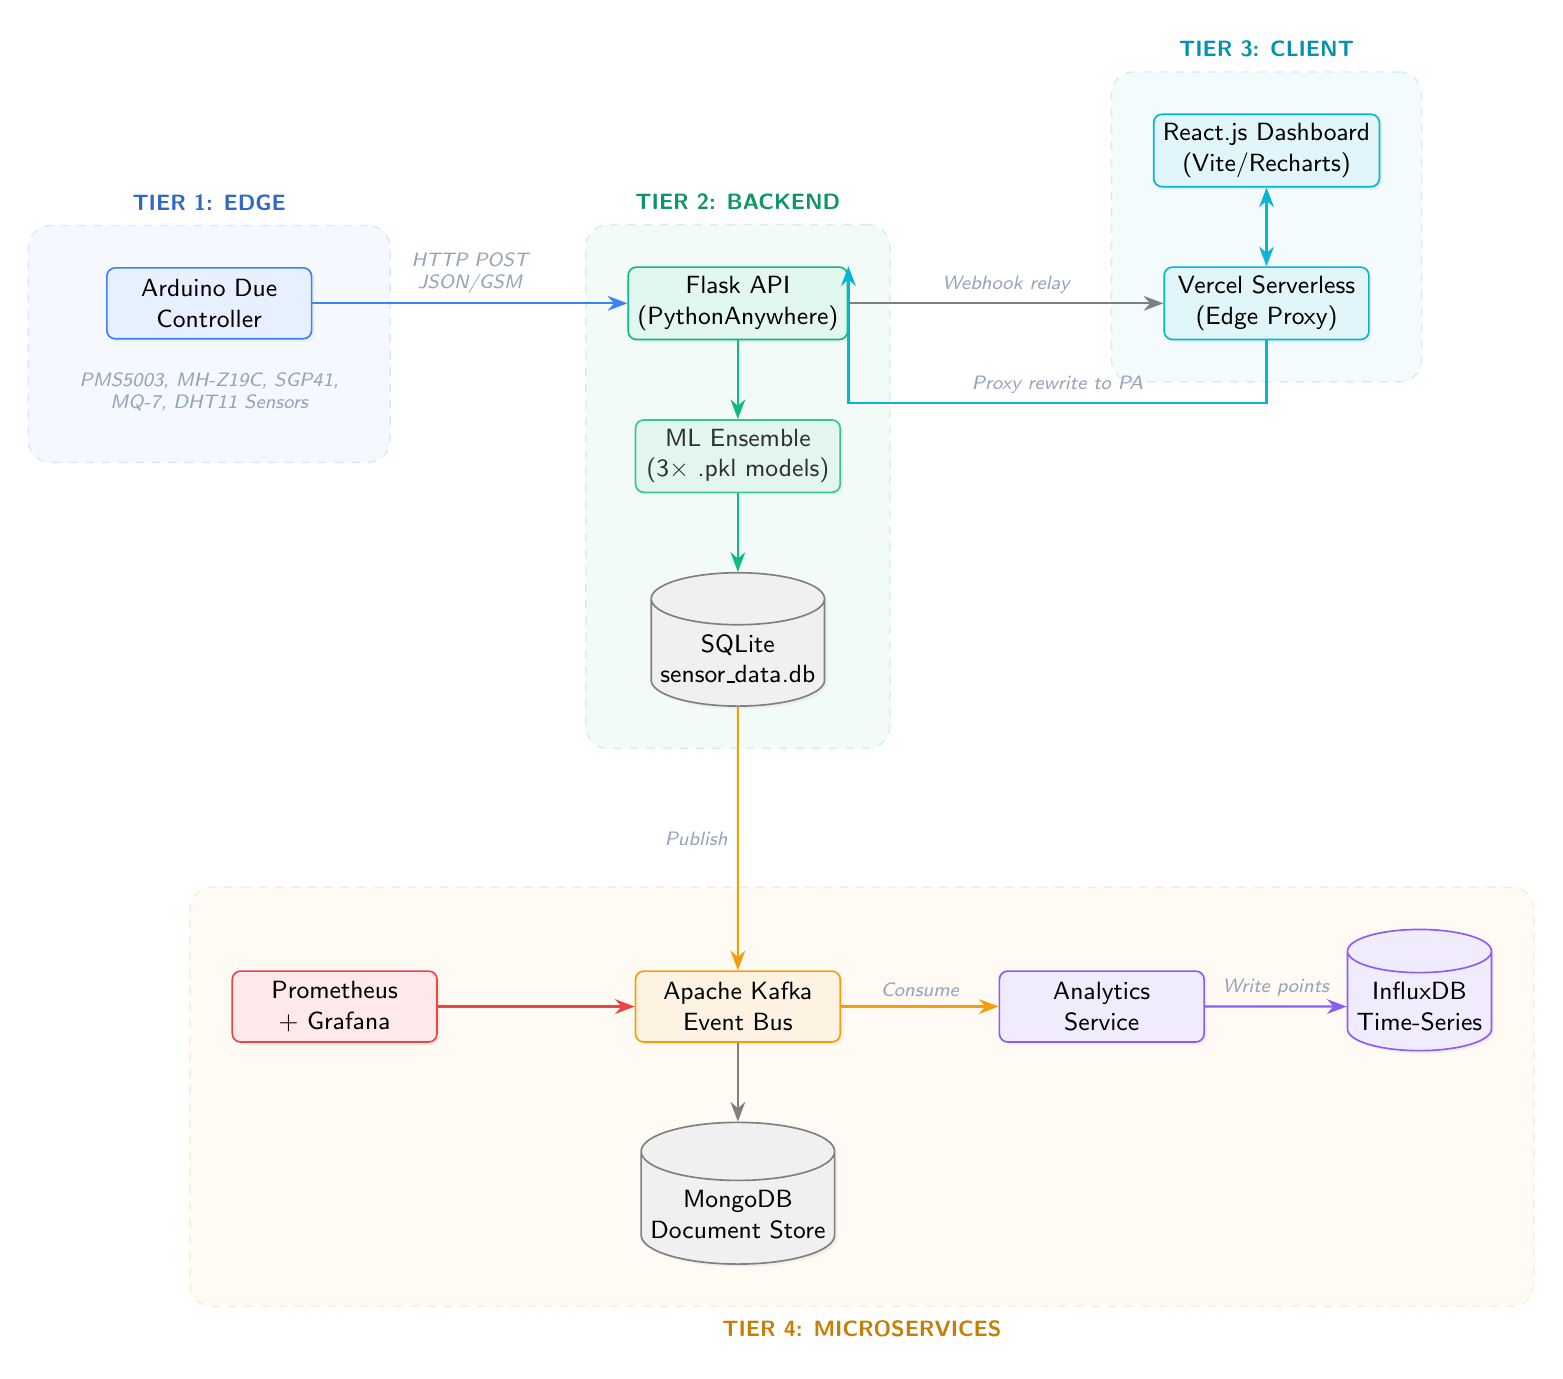
\begin{tikzpicture}[node distance=1.5cm and 2.5cm]

\node[sysblock=edgeblue] (arduino) {Arduino Due\\Controller};
\node[below=0.3cm of arduino, sysannot] (sensors) {PMS5003, MH-Z19C, SGP41,\\MQ-7, DHT11 Sensors};

\node[sysblock=flaskgreen, right=4cm of arduino] (flask) {Flask API\\(PythonAnywhere)};
\node[sysblock=flaskgreen, below=1cm of flask, opacity=0.8] (ml) {ML Ensemble\\(3$\times$ .pkl models)};
\node[sysdb=gray, below=1cm of ml] (sqlite) {SQLite\\sensor\_data.db};

\node[sysblock=reactcyan, right=4cm of flask] (vercel) {Vercel Serverless\\(Edge Proxy)};
\node[sysblock=reactcyan, above=1cm of vercel] (react) {React.js Dashboard\\(Vite/Recharts)};

\node[sysblock=kafkaorange, below=8cm of flask] (kafka) {Apache Kafka\\Event Bus};
\node[sysblock=influxpurple, right=2cm of kafka] (analytics) {Analytics\\Service};
\node[sysdb=influxpurple, right=1.8cm of analytics] (influx) {InfluxDB\\Time-Series};
\node[sysdb=gray, below=1cm of kafka] (mongo) {MongoDB\\Document Store};
\node[sysblock=dangered, left=2.5cm of kafka] (prom) {Prometheus\\+ Grafana};

\draw[sysarrow, edgeblue] (arduino) -- node[above, sysannot] {HTTP POST\\JSON/GSM} (flask);
\draw[sysarrow, flaskgreen] (flask) -- (ml);
\draw[sysarrow, flaskgreen] (ml) -- (sqlite);
\draw[sysarrow, gray] (flask) -- node[above, sysannot] {Webhook relay} (vercel);
\draw[sysdarrow, reactcyan] (vercel) -- (react);
\draw[sysarrow, reactcyan] (vercel.south) -- ++(0,-0.8) -| node[near start, above, sysannot] {Proxy rewrite to PA} (flask.north east);
\draw[sysarrow, kafkaorange] (sqlite.south) -- node[left, sysannot] {Publish} (kafka.north);
\draw[sysarrow, kafkaorange] (kafka) -- node[above, sysannot] {Consume} (analytics);
\draw[sysarrow, influxpurple] (analytics) -- node[above, sysannot] {Write points} (influx);
\draw[sysarrow, gray] (kafka) -- (mongo);
\draw[sysarrow, dangered] (prom) -- (kafka);

\begin{scope}[on background layer]
    \node[syscontainer=edgeblue, fit=(arduino) (sensors), label={[systier=edgeblue]above:TIER 1: EDGE}] {};
    \node[syscontainer=flaskgreen, fit=(flask) (ml) (sqlite), label={[systier=flaskgreen]above:TIER 2: BACKEND}] {};
    \node[syscontainer=reactcyan, fit=(vercel) (react), label={[systier=reactcyan]above:TIER 3: CLIENT}] {};
    \node[syscontainer=kafkaorange, fit=(kafka) (analytics) (influx) (mongo) (prom), label={[systier=kafkaorange]below:TIER 4: MICROSERVICES}] {};
\end{scope}

\end{tikzpicture}%
}
\caption{Complete AQMRG platform architecture showing the multi-tier data flow. Tiers are logically grouped by role, spanning from edge sensing to cloud-hosted analytics and event streaming via Apache Kafka.}
\label{fig:arch}
\end{figure}

\begin{figure}[H]
\centering
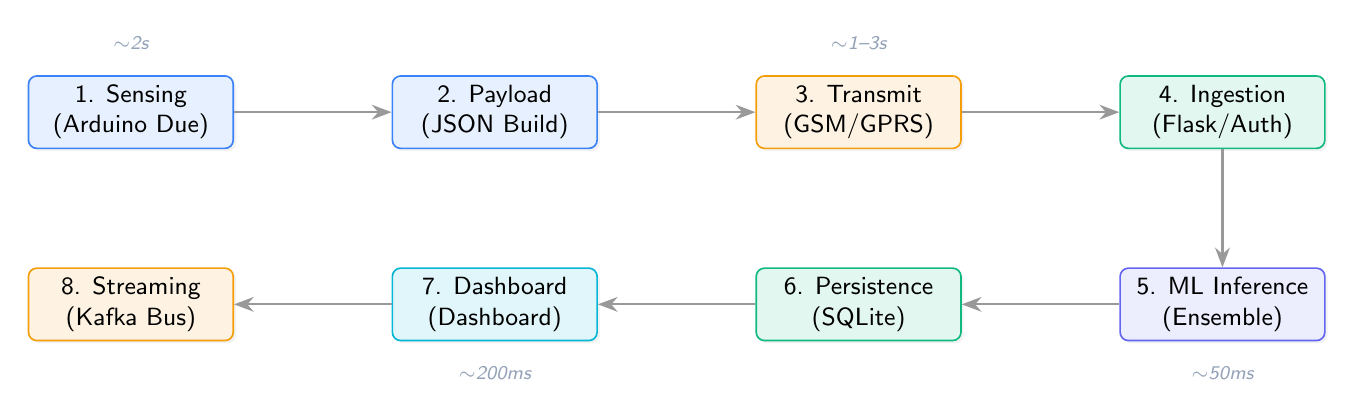
\begin{tikzpicture}[node distance=1cm and 2cm]

\node[sysblock=edgeblue] (p1) {1. Sensing\\(Arduino Due)};
\node[sysblock=edgeblue, right=of p1] (p2) {2. Payload\\(JSON Build)};
\node[sysblock=amber, right=of p2] (p3) {3. Transmit\\(GSM/GPRS)};
\node[sysblock=flaskgreen, right=of p3] (p4) {4. Ingestion\\(Flask/Auth)};

\node[sysblock=indigo, below=1.5cm of p4] (p5) {5. ML Inference\\(Ensemble)};
\node[sysblock=flaskgreen, left=of p5] (p6) {6. Persistence\\(SQLite)};
\node[sysblock=reactcyan, left=of p6] (p7) {7. Dashboard\\(Dashboard)};
\node[sysblock=kafkaorange, left=of p7] (p8) {8. Streaming\\(Kafka Bus)};

\draw[sysarrow] (p1) -- (p2);
\draw[sysarrow] (p2) -- (p3);
\draw[sysarrow] (p3) -- (p4);
\draw[sysarrow] (p4) -- (p5);
\draw[sysarrow] (p5) -- (p6);
\draw[sysarrow] (p6) -- (p7);
\draw[sysarrow] (p7) -- (p8);

\node[sysannot, above=0.2cm of p1] {$\sim$2s};
\node[sysannot, above=0.2cm of p3] {$\sim$1--3s};
\node[sysannot, below=0.2cm of p5] {$\sim$50ms};
\node[sysannot, below=0.2cm of p7] {$\sim$200ms};

\end{tikzpicture}
\caption{End-to-end data lifecycle in a compact snaking layout. Timing annotations indicate typical systemic latency from physical sensing to global dashboard availability.}
\label{fig:lifecycle}
\end{figure}

\begin{figure}[H]
\centering
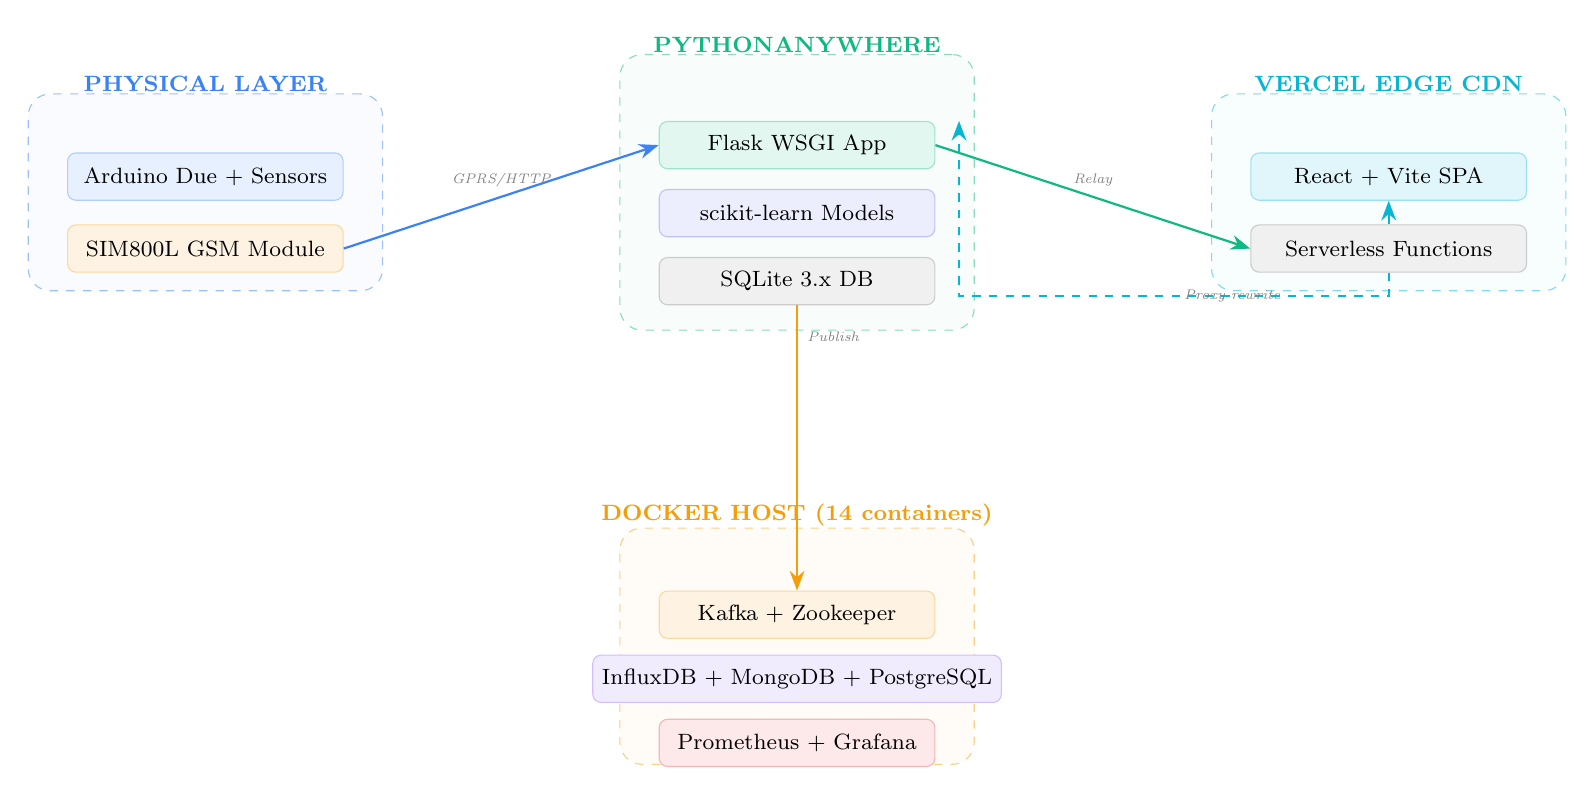
\begin{tikzpicture}[
    every node/.style={font=\small},
    cloudbox/.style={rectangle, draw, rounded corners=8pt, minimum width=4.5cm, minimum height=2cm, align=center, dashed, draw=#1!50, fill=#1!3},
    innerblock/.style={rectangle, draw, rounded corners=3pt, minimum width=3.5cm, minimum height=0.6cm, align=center, font=\footnotesize, fill=#1!12, draw=#1!40},
    arrow/.style={-{Stealth[length=2.5mm]}, thick}
]

\node[cloudbox=edgeblue, minimum height=2.5cm] (physical) at (0,0) {};
\node[above=-0.1cm of physical.north, font=\footnotesize\bfseries, text=edgeblue] {PHYSICAL LAYER};
\node[innerblock=edgeblue] (ard) at (0, 0.2) {Arduino Due + Sensors};
\node[innerblock=amber, below=0.3cm of ard] (gsm) {SIM800L GSM Module};

\node[cloudbox=flaskgreen, minimum height=3.5cm, right=3cm of physical] (pacloud) {};
\node[above=-0.1cm of pacloud.north, font=\footnotesize\bfseries, text=flaskgreen] {PYTHONANYWHERE};
\node[innerblock=flaskgreen] (flaskd) at ([yshift=0.6cm]pacloud.center) {Flask WSGI App};
\node[innerblock=indigo, below=0.25cm of flaskd] (mld) {scikit-learn Models};
\node[innerblock=gray, below=0.25cm of mld] (sqld) {SQLite 3.x DB};

\node[cloudbox=reactcyan, minimum height=2.5cm, right=3cm of pacloud] (vercelcloud) {};
\node[above=-0.1cm of vercelcloud.north, font=\footnotesize\bfseries, text=reactcyan] {VERCEL EDGE CDN};
\node[innerblock=reactcyan] (reactd) at ([yshift=0.2cm]vercelcloud.center) {React + Vite SPA};
\node[innerblock=gray, below=0.3cm of reactd] (sless) {Serverless Functions};

\node[cloudbox=kafkaorange, minimum height=3cm, below=2.5cm of pacloud] (docker) {};
\node[above=-0.1cm of docker.north, font=\footnotesize\bfseries, text=kafkaorange] {DOCKER HOST (14 containers)};
\node[innerblock=kafkaorange] (kd) at ([yshift=0.4cm]docker.center) {Kafka + Zookeeper};
\node[innerblock=influxpurple, below=0.2cm of kd] (idb) {InfluxDB + MongoDB + PostgreSQL};
\node[innerblock=dangered, below=0.2cm of idb] (obd) {Prometheus + Grafana};

\draw[arrow, edgeblue] (gsm.east) -- node[above, font=\tiny\itshape, text=gray] {GPRS/HTTP} (flaskd.west);
\draw[arrow, flaskgreen] (flaskd.east) -- node[above, font=\tiny\itshape, text=gray] {Relay} (sless.west);
\draw[arrow, reactcyan] (sless) -- (reactd);
\draw[arrow, kafkaorange] (sqld.south) -- ++(0,-0.4) -| node[near start, right, font=\tiny\itshape, text=gray] {Publish} (kd.north);
\draw[arrow, reactcyan, dashed] (sless.south) -- ++(0,-0.3) -| node[near start, right, font=\tiny\itshape, text=gray] {Proxy rewrite} ([xshift=0.3cm]flaskd.north east);

\end{tikzpicture}
\caption{Physical deployment topology showing the four hosting environments: a field-deployed Arduino node, PythonAnywhere's managed Python hosting, Vercel's edge CDN, and a Docker Compose cluster for microservices.}
\label{fig:deploy}
\end{figure}

\section{Edge Hardware Tier: Arduino Due Sensor Node}

\subsection{Microcontroller Selection}
The Arduino Due, based on the Atmel SAM3X8E ARM Cortex-M3 processor operating at 84~MHz with 96~KB SRAM, was selected for its multiple hardware serial ports (enabling simultaneous communication with UART-based sensors) and its 3.3~V logic level compatibility with modern sensor modules. Table~\ref{tab:mcu} summarizes the key specifications.

\begin{table}[H]
\centering
\caption{Arduino Due microcontroller specifications.}
\label{tab:mcu}
\begin{tabular}{@{}ll@{}}
\toprule
\textbf{Specification} & \textbf{Value} \\
\midrule
Processor & Atmel SAM3X8E (ARM Cortex-M3) \\
Clock Speed & 84 MHz \\
SRAM & 96 KB \\
Flash Memory & 512 KB \\
Logic Level & 3.3 V \\
Hardware Serial Ports & 4 (Serial, Serial1, Serial2, Serial3) \\
I$^2$C Buses & 2 (TWI0, TWI1) \\
Analog Inputs & 12 channels (12-bit ADC) \\
Operating Voltage & 3.3 V (5V barrel jack input) \\
\bottomrule
\end{tabular}
\end{table}

\subsection{Sensor Array Composition}
Each edge node integrates five dedicated environmental sensors, summarized in Table~\ref{tab:sensors}.

\begin{table}[H]
\centering
\caption{Hardware sensor array configuration per AQMRG edge node.}
\label{tab:sensors}
\begin{tabular}{@{}llllp{3cm}@{}}
\toprule
\textbf{Sensor} & \textbf{Parameters} & \textbf{Interface} & \textbf{Principle} & \textbf{Range / Resolution} \\
\midrule
PMS5003 & $PM_1$, $PM_{2.5}$, $PM_{10}$ & UART (Serial3) & Laser scattering & 0--500 $\mu$g/m$^3$ / 1 $\mu$g/m$^3$ \\
MH-Z19C & CO$_2$ (ppm) & UART (Serial2) & NDIR absorption & 0--5000 ppm / $\pm$50 ppm \\
SGP41 & VOC Index, NO$_x$ Index & I$^2$C (SDA/SCL) & MOx hotplate & 0--500 index / 1 unit \\
MQ-7 & CO (ppm) & Analog (A0) & Electrochemical & 10--500 ppm / variable \\
DHT11 & Temperature, Humidity & Digital (Pin 7) & Capacitive & 0--50$^\circ$C, 20--90\% RH \\
\bottomrule
\end{tabular}
\end{table}

\begin{figure}[H]
\centering
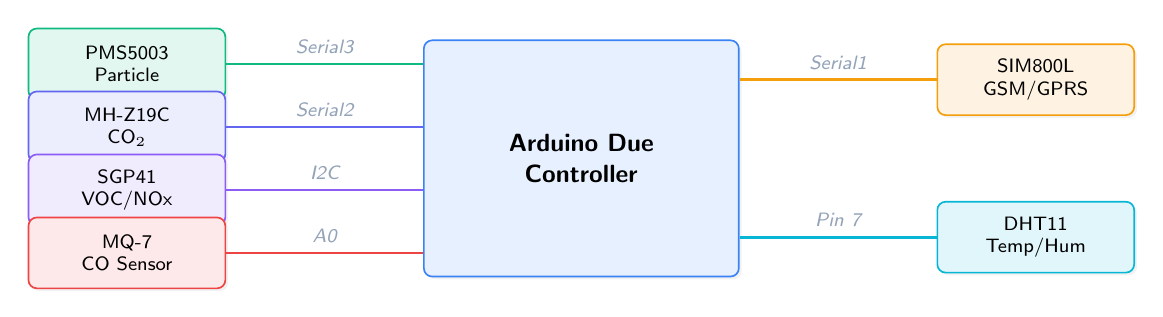
\begin{tikzpicture}[
    node distance=1cm and 2.5cm,
    sensor/.style={sysblock=#1, minimum width=2.5cm, font=\sffamily\scriptsize},
    bus/.style={draw=#1, thick, line width=1pt}
]

\node[sysblock=edgeblue, minimum width=4cm, minimum height=3cm] (mcu) {\textbf{Arduino Due}\\\textbf{Controller}};

\node[sensor=flaskgreen, left=of mcu, yshift=1.2cm] (pms) {PMS5003\\Particle};
\node[sensor=indigo, left=of mcu, yshift=0.4cm] (mhz) {MH-Z19C\\CO$_2$};
\node[sensor=influxpurple, left=of mcu, yshift=-0.4cm] (sgp) {SGP41\\VOC/NOx};
\node[sensor=dangered, left=of mcu, yshift=-1.2cm] (mq7) {MQ-7\\CO Sensor};

\node[sensor=amber, right=of mcu, yshift=1cm] (gsm) {SIM800L\\GSM/GPRS};
\node[sensor=reactcyan, right=of mcu, yshift=-1cm] (dht) {DHT11\\Temp/Hum};

\draw[bus=flaskgreen] (pms.east) -- node[above, sysannot] {Serial3} (mcu.west |- pms.east);
\draw[bus=indigo] (mhz.east) -- node[above, sysannot] {Serial2} (mcu.west |- mhz.east);
\draw[bus=influxpurple] (sgp.east) -- node[above, sysannot] {I2C} (mcu.west |- sgp.east);
\draw[bus=dangered] (mq7.east) -- node[above, sysannot] {A0} (mcu.west |- mq7.east);
\draw[bus=amber] (gsm.west) -- node[above, sysannot] {Serial1} (mcu.east |- gsm.west);
\draw[bus=reactcyan] (dht.west) -- node[above, sysannot] {Pin 7} (mcu.east |- dht.west);

\end{tikzpicture}
\caption{Hardware wiring topology. Sensor modules connect to the Arduino Due via diverse interfaces (UART, I2C, Analog, Digital), with the SIM800L module providing cellular connectivity.}
\label{fig:wiring}
\end{figure}

\subsection{Payload Construction and Transmission}
The firmware executes a continuous polling loop, sampling all five sensors and constructing a structured JSON payload containing three nested objects:
\begin{itemize}[nosep]
    \item \textbf{metrics}: Numerical sensor readings ($PM_1$, $PM_{2.5}$, $PM_{10}$, CO, CO$_2$, temperature, humidity, VOC index, NO$_x$ index).
    \item \textbf{location}: GPS-fixed latitude and longitude coordinates for geographic tagging.
    \item \textbf{health}: Diagnostic telemetry including system uptime (minutes), GSM signal strength (dBm), GSM reconnection count, failed HTTP request count, last HTTP status code, and per-sensor operational status flags.
\end{itemize}

Each device is assigned a unique hardware identifier with the \texttt{AQ-} prefix (e.g., \texttt{AQ-001}). The payload is transmitted as an HTTP POST request over a SIM800L GSM/GPRS module to the Flask backend endpoint \texttt{/api/v1/data/ingest} on the PythonAnywhere server. A hardware authentication lock in the backend silently rejects any payload whose \texttt{device\_id} does not begin with the \texttt{AQ-} prefix, protecting the database from unauthorized or spoofed submissions.

\begin{figure}[H]
\centering
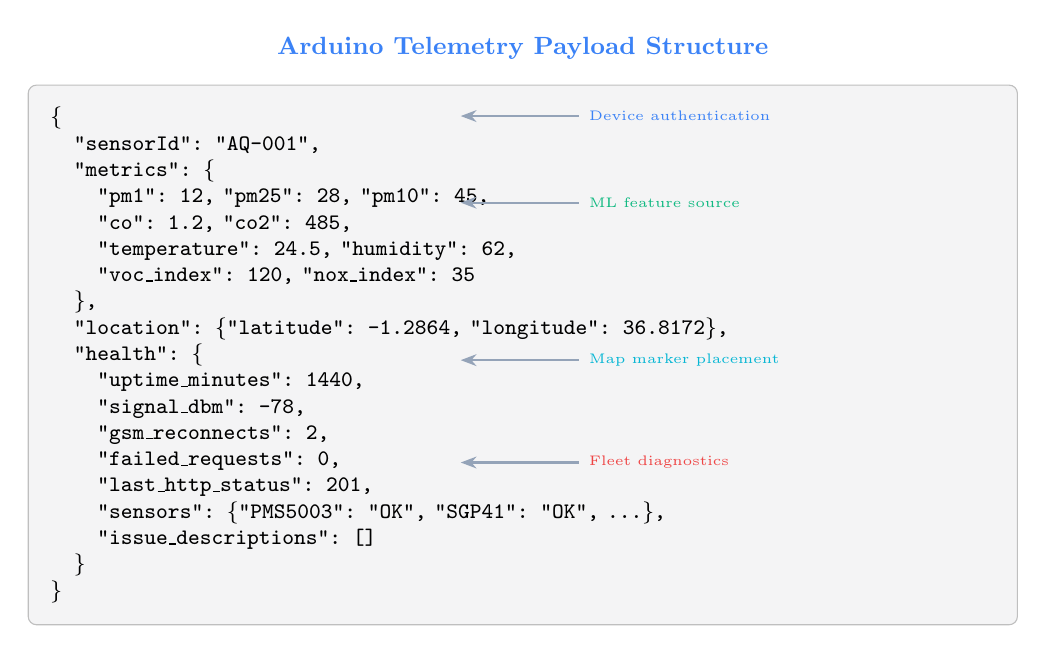
\begin{tikzpicture}[
    every node/.style={font=\footnotesize},
    jsonblock/.style={rectangle, draw=gray!50, fill=darkslate!5, rounded corners=3pt, minimum width=5cm, align=left, inner sep=8pt}
]

\node[jsonblock, text width=12cm] (json) {
\texttt{\{}\\
\quad\texttt{"sensorId": "AQ-001",}\\
\quad\texttt{"metrics": \{}\\
\quad\quad\texttt{"pm1": 12, "pm25": 28, "pm10": 45,}\\
\quad\quad\texttt{"co": 1.2, "co2": 485,}\\
\quad\quad\texttt{"temperature": 24.5, "humidity": 62,}\\
\quad\quad\texttt{"voc\_index": 120, "nox\_index": 35}\\
\quad\texttt{\},}\\
\quad\texttt{"location": \{"latitude": -1.2864, "longitude": 36.8172\},}\\
\quad\texttt{"health": \{}\\
\quad\quad\texttt{"uptime\_minutes": 1440,}\\
\quad\quad\texttt{"signal\_dbm": -78,}\\
\quad\quad\texttt{"gsm\_reconnects": 2,}\\
\quad\quad\texttt{"failed\_requests": 0,}\\
\quad\quad\texttt{"last\_http\_status": 201,}\\
\quad\quad\texttt{"sensors": \{"PMS5003": "OK", "SGP41": "OK", ...\},}\\
\quad\quad\texttt{"issue\_descriptions": []}\\
\quad\texttt{\}}\\
\texttt{\}}
};

\node[above=0.2cm of json, font=\small\bfseries, text=edgeblue] {Arduino Telemetry Payload Structure};

\draw[{Stealth[length=2mm]}-, thick, softgray] ([xshift=5.5cm, yshift=-0.4cm]json.north west) -- ++(1.5,0) node[right, font=\tiny, text=edgeblue] {Device authentication};
\draw[{Stealth[length=2mm]}-, thick, softgray] ([xshift=5.5cm, yshift=-1.5cm]json.north west) -- ++(1.5,0) node[right, font=\tiny, text=flaskgreen] {ML feature source};
\draw[{Stealth[length=2mm]}-, thick, softgray] ([xshift=5.5cm, yshift=-3.5cm]json.north west) -- ++(1.5,0) node[right, font=\tiny, text=reactcyan] {Map marker placement};
\draw[{Stealth[length=2mm]}-, thick, softgray] ([xshift=5.5cm, yshift=-4.8cm]json.north west) -- ++(1.5,0) node[right, font=\tiny, text=dangered] {Fleet diagnostics};

\end{tikzpicture}
\caption{Structure of the JSON telemetry payload transmitted from the Arduino Due to the Flask backend. Annotations indicate which downstream subsystem consumes each section.}
\label{fig:payload}
\end{figure}

\begin{figure}[H]
\centering
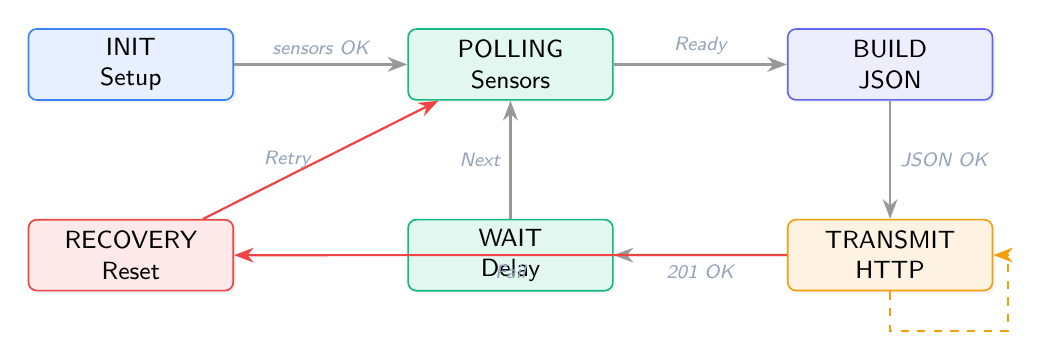
\begin{tikzpicture}[node distance=1.2cm and 2.2cm]

\node[sysblock=edgeblue] (init) {INIT\\Setup};
\node[sysblock=flaskgreen, right=of init] (sensor) {POLLING\\Sensors};
\node[sysblock=indigo, right=of sensor] (build) {BUILD\\JSON};
\node[sysblock=amber, below=1.5cm of build] (gsm) {TRANSMIT\\HTTP};
\node[sysblock=flaskgreen, below=1.5cm of sensor] (wait) {WAIT\\Delay};
\node[sysblock=dangered, below=1.5cm of init] (error) {RECOVERY\\Reset};

\draw[sysarrow] (init) -- node[above, sysannot] {sensors OK} (sensor);
\draw[sysarrow] (sensor) -- node[above, sysannot] {Ready} (build);
\draw[sysarrow] (build) -- node[right, sysannot] {JSON OK} (gsm);
\draw[sysarrow] (gsm) -- node[below, sysannot] {201 OK} (wait);
\draw[sysarrow] (wait) -- node[left, sysannot] {Next} (sensor);
\draw[sysarrow, dangered] (gsm.west) -- node[below, sysannot] {Fail} (error);
\draw[sysarrow, dangered] (error) -- node[left, sysannot] {Retry} (sensor);

\draw[sysarrow, dashed, amber] (gsm.south) -- ++(0,-0.5) -- ++(1.5,0) |- (gsm.east);

\end{tikzpicture}
\caption{Firmware state machine governing the operational lifecycle of the edge node, including polling cycles and fault recovery logic.}
\label{fig:firmware_fsm}
\end{figure}

\section{Primary Backend Tier: Flask API on PythonAnywhere}

\subsection{Application Framework}
The backend is implemented as a Python Flask application utilizing SQLAlchemy as an Object-Relational Mapper (ORM). The application factory pattern (\texttt{create\_app}) initializes the database connection, registers API blueprints, integrates Swagger/Flasgger for automatic API documentation, and applies a critical SQLite stability fix for PythonAnywhere's Network File System (NFS) by forcing \texttt{PRAGMA journal\_mode=DELETE} to prevent write-ahead log (WAL) corruption on distributed filesystems.

\begin{figure}[H]
\centering
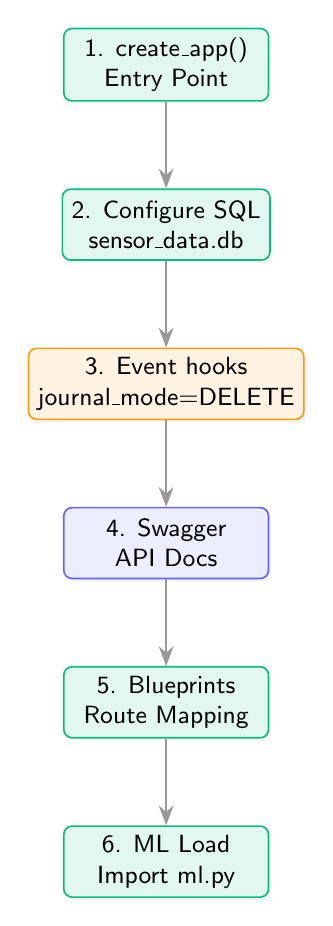
\begin{tikzpicture}[node distance=1.1cm]

\node[sysblock=flaskgreen] (s1) {1. create\_app()\\Entry Point};
\node[sysblock=flaskgreen, below=of s1] (s2) {2. Configure SQL\\sensor\_data.db};
\node[sysblock=amber, below=of s2] (s3) {3. Event hooks\\journal\_mode=DELETE};
\node[sysblock=indigo, below=of s3] (s4) {4. Swagger\\API Docs};
\node[sysblock=flaskgreen, below=of s4] (s5) {5. Blueprints\\Route Mapping};
\node[sysblock=emerald, below=of s5] (s6) {6. ML Load\\Import ml.py};

\draw[sysarrow] (s1) -- (s2);
\draw[sysarrow] (s2) -- (s3);
\draw[sysarrow] (s3) -- (s4);
\draw[sysarrow] (s4) -- (s5);
\draw[sysarrow] (s5) -- (s6);

\end{tikzpicture}
\caption{Flask application factory initialization flow. The system utilizes a singleton pattern for ML model loading during the WSGI server startup phase.}
\label{fig:app_factory}
\end{figure}

\subsection{Relational Data Schema}
The SQLite database (\texttt{sensor\_data.db}, currently 6.16~MB in production) contains three ORM-mapped tables. Figure~\ref{fig:erd} illustrates the Entity-Relationship diagram.

\begin{figure}[H]
\centering
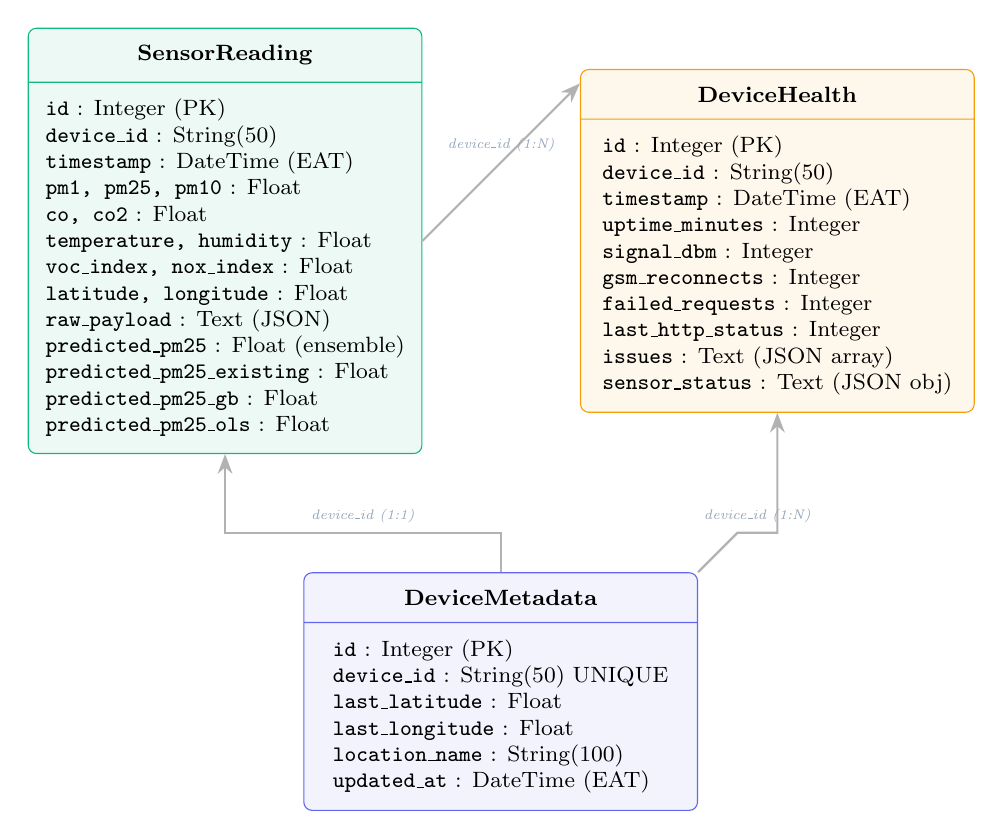
\begin{tikzpicture}[
    every node/.style={font=\small},
    entity/.style={rectangle split, rectangle split parts=2, draw=#1, fill=#1!8, rounded corners=3pt, minimum width=5cm, align=left, font=\footnotesize, inner sep=6pt},
    arrow/.style={-{Stealth[length=2.5mm]}, thick, gray!60},
    rel/.style={font=\tiny\itshape, text=softgray}
]

\node[entity=flaskgreen] (sr) {
    \textbf{SensorReading}
    \nodepart{second}
    \texttt{id} : Integer (PK)\\
    \texttt{device\_id} : String(50)\\
    \texttt{timestamp} : DateTime (EAT)\\
    \texttt{pm1, pm25, pm10} : Float\\
    \texttt{co, co2} : Float\\
    \texttt{temperature, humidity} : Float\\
    \texttt{voc\_index, nox\_index} : Float\\
    \texttt{latitude, longitude} : Float\\
    \texttt{raw\_payload} : Text (JSON)\\
    \texttt{predicted\_pm25} : Float (ensemble)\\
    \texttt{predicted\_pm25\_existing} : Float\\
    \texttt{predicted\_pm25\_gb} : Float\\
    \texttt{predicted\_pm25\_ols} : Float
};

\node[entity=amber, right=2cm of sr] (dh) {
    \textbf{DeviceHealth}
    \nodepart{second}
    \texttt{id} : Integer (PK)\\
    \texttt{device\_id} : String(50)\\
    \texttt{timestamp} : DateTime (EAT)\\
    \texttt{uptime\_minutes} : Integer\\
    \texttt{signal\_dbm} : Integer\\
    \texttt{gsm\_reconnects} : Integer\\
    \texttt{failed\_requests} : Integer\\
    \texttt{last\_http\_status} : Integer\\
    \texttt{issues} : Text (JSON array)\\
    \texttt{sensor\_status} : Text (JSON obj)
};

\node[entity=indigo, below=1.5cm of sr, xshift=3.5cm] (dm) {
    \textbf{DeviceMetadata}
    \nodepart{second}
    \texttt{id} : Integer (PK)\\
    \texttt{device\_id} : String(50) UNIQUE\\
    \texttt{last\_latitude} : Float\\
    \texttt{last\_longitude} : Float\\
    \texttt{location\_name} : String(100)\\
    \texttt{updated\_at} : DateTime (EAT)
};

\draw[arrow] (sr.east) -- node[above, rel] {device\_id (1:N)} ([yshift=2cm]dh.west);
\draw[arrow] (dm.north) -- ++(0,0.5) -| node[near start, above, rel] {device\_id (1:1)} (sr.south);
\draw[arrow] (dm.north east) -- ++(0.5,0.5) -| node[near start, above, rel] {device\_id (1:N)} (dh.south);

\end{tikzpicture}
\caption{Entity-Relationship diagram for the SQLite database. Each \texttt{SensorReading} stores raw sensor data plus all four prediction columns. \texttt{DeviceHealth} provides per-submission hardware diagnostics, and \texttt{DeviceMetadata} maintains persistent geographic identity per device.}
\label{fig:erd}
\end{figure}

\subsection{Ingestion Pipeline and Real-Time ML Inference}
The ingestion endpoint (\texttt{POST /api/v1/data/ingest}) implements the following sequential logic upon receiving a valid \texttt{AQ-} prefixed payload:

\begin{enumerate}[nosep]
    \item \textbf{Device Authentication}: Verify that \texttt{device\_id} starts with \texttt{AQ-} prefix; silently reject unauthorized devices with HTTP 200 (preventing enumeration).
    \item \textbf{Feature Extraction}: Parse the \texttt{metrics} object to extract the four ML input features: $PM_{10}$, CO, Temperature, and Humidity.
    \item \textbf{Parallel Model Inference}: Pass the feature vector $\mathbf{x} = [PM_{10}, CO, T, H]$ simultaneously through three pre-loaded scikit-learn models (see Section~\ref{sec:ml}).
    \item \textbf{Ensemble Aggregation}: Compute the median of all successful (non-null) predictions to produce the ensemble forecast.
    \item \textbf{Database Persistence}: Write a \texttt{SensorReading} row containing raw observations, all three individual predictions, and the ensemble value. If health data is present, simultaneously write a \texttt{DeviceHealth} row.
    \item \textbf{Dashboard Relay}: Issue an asynchronous HTTP POST forwarding the original payload to the Vercel frontend's ingestion endpoint (\texttt{aqmrg-frontend.vercel.app/api/v1/data/ingest}) with a 3-second timeout to prevent blocking.
    \item \textbf{Response}: Return \texttt{\{status: "success", id: N\}} with HTTP 201 to the Arduino.
\end{enumerate}

\begin{figure}[H]
\centering
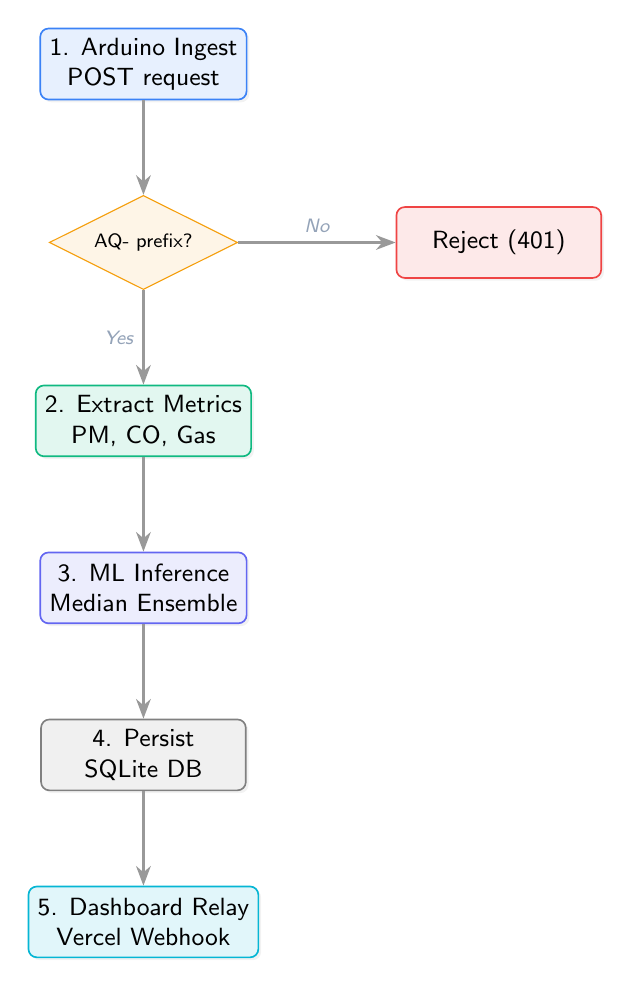
\begin{tikzpicture}[node distance=1.2cm]

\node[sysblock=edgeblue] (s1) {1. Arduino Ingest\\POST request};
\node[diamond, draw=amber, fill=amber!10, below=of s1, aspect=2, align=center, font=\sffamily\scriptsize] (d1) {AQ- prefix?};
\node[sysblock=dangered, right=2cm of d1] (reject) {Reject (401)};
\node[sysblock=flaskgreen, below=of d1] (s2) {2. Extract Metrics\\PM, CO, Gas};
\node[sysblock=indigo, below=of s2] (s3) {3. ML Inference\\Median Ensemble};
\node[sysblock=gray, below=of s3] (s4) {4. Persist\\SQLite DB};
\node[sysblock=reactcyan, below=of s4] (s5) {5. Dashboard Relay\\Vercel Webhook};

\draw[sysarrow] (s1) -- (d1);
\draw[sysarrow] (d1) -- node[above, sysannot] {No} (reject);
\draw[sysarrow] (d1) -- node[left, sysannot] {Yes} (s2);
\draw[sysarrow] (s2) -- (s3);
\draw[sysarrow] (s3) -- (s4);
\draw[sysarrow] (s4) -- (s5);

\end{tikzpicture}
\caption{Ingestion pipeline logic flow. Each request is validated, passed through the ML ensemble, and asynchronously relayed to the live dashboard within the HTTP cycle.}
\label{fig:ingest}
\end{figure}

\subsection{API Endpoint Inventory}

\begin{table}[H]
\centering
\caption{Complete REST API endpoints exposed by the Flask backend.}
\label{tab:endpoints}
\begin{tabular}{@{}llp{6.5cm}@{}}
\toprule
\textbf{Method} & \textbf{Endpoint} & \textbf{Function} \\
\midrule
POST & \texttt{/api/v1/data/ingest} & Primary ingestion from Arduino; runs ML, persists, relays. \\
GET & \texttt{/api/v1/data/latest} & Returns last 100 readings (filterable by \texttt{device\_id}). \\
GET & \texttt{/api/v1/history/all} & Returns full historical dataset for EDA. \\
GET & \texttt{/api/v1/devices} & Lists all registered \texttt{AQ-} devices with coordinates. \\
GET & \texttt{/api/v1/forecast/realtime} & Returns latest ensemble prediction vs.\ actual reading. \\
GET & \texttt{/api/v1/forecast/comparison} & Returns all three model predictions plus ensemble median. \\
GET & \texttt{/api/v1/health/latest} & Returns device health diagnostics. \\
GET & \texttt{/api/v1/data/export/csv} & Downloads complete sensor data as CSV. \\
GET & \texttt{/api/v1/health/export/csv} & Downloads health diagnostics as CSV. \\
GET & \texttt{/health} & Service health check. \\
\bottomrule
\end{tabular}
\end{table}

\section{Machine Learning Methodology}
\label{sec:ml}

\subsection{Problem Formulation}
The prediction task is formulated as a supervised regression problem: given the input feature vector $\mathbf{x} = [PM_{10},\ CO,\ T,\ H]$ derived from co-located sensor readings, predict the concurrent $PM_{2.5}$ concentration $\hat{y}$. This formulation exploits the physical correlations between coarse particulate fractions, trace gas emissions from common combustion sources, and meteorological conditions that govern aerosol behaviour.

\subsection{Training Data}
Models were trained on the AQMRG relay dataset (\texttt{aqmrg\_relay\_data\_20260309.csv}, 147~KB) collected from the Nairobi deployment. The training pipeline is documented in the Jupyter notebook \texttt{ml/aqmrg\_air\_quality\_prediction.ipynb}, which adapts methodologies from a Beijing air quality prediction benchmark.

\begin{figure}[H]
\centering
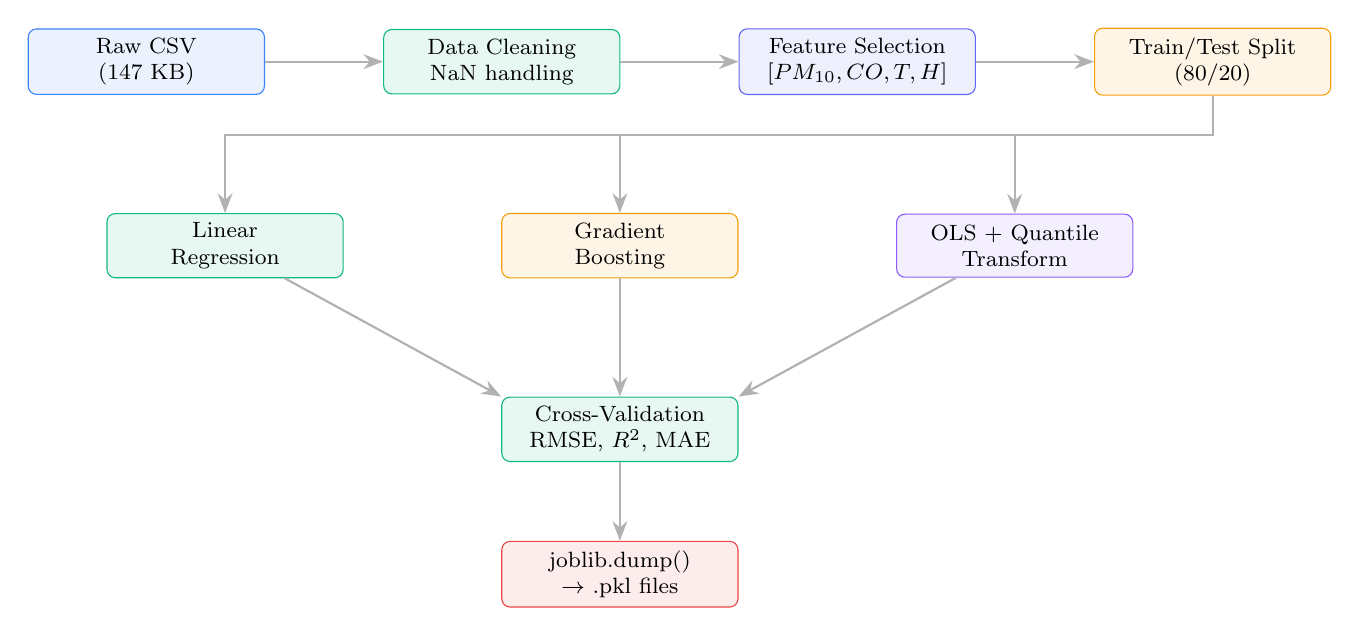
\begin{tikzpicture}[
    every node/.style={font=\small},
    block/.style={rectangle, draw=#1, fill=#1!10, rounded corners=3pt, minimum width=3cm, minimum height=0.8cm, align=center, font=\footnotesize},
    arrow/.style={-{Stealth[length=2.5mm]}, thick, gray!60}
]

\node[block=edgeblue] (raw) {Raw CSV\\(147 KB)};
\node[block=flaskgreen, right=1.5cm of raw] (clean) {Data Cleaning\\NaN handling};
\node[block=indigo, right=1.5cm of clean] (feat) {Feature Selection\\$[PM_{10}, CO, T, H]$};
\node[block=amber, right=1.5cm of feat] (split) {Train/Test Split\\(80/20)};

\node[block=flaskgreen, below=1.5cm of raw, xshift=1cm] (lr) {Linear\\Regression};
\node[block=kafkaorange, right=2cm of lr] (gb) {Gradient\\Boosting};
\node[block=influxpurple, right=2cm of gb] (ols) {OLS + Quantile\\Transform};

\node[block=emerald, below=1.5cm of gb] (eval) {Cross-Validation\\RMSE, $R^2$, MAE};
\node[block=dangered, below=1cm of eval] (serial) {joblib.dump()\\$\rightarrow$ .pkl files};

\draw[arrow] (raw) -- (clean);
\draw[arrow] (clean) -- (feat);
\draw[arrow] (feat) -- (split);

\draw[arrow] (split.south) -- ++(0,-0.5) -| (lr.north);
\draw[arrow] (split.south) -- ++(0,-0.5) -| (gb.north);
\draw[arrow] (split.south) -- ++(0,-0.5) -| (ols.north);

\draw[arrow] (lr) -- (eval.north west);
\draw[arrow] (gb) -- (eval);
\draw[arrow] (ols) -- (eval.north east);
\draw[arrow] (eval) -- (serial);

\end{tikzpicture}
\caption{ML training pipeline: raw CSV data undergoes cleaning and feature selection before being split into training/test sets. Three distinct algorithms are trained, cross-validated, and serialized for production deployment.}
\label{fig:training_pipeline}
\end{figure}

\subsection{Model Architectures}
Three distinct regression algorithms were trained, evaluated, and serialized as \texttt{.pkl} files using joblib for production deployment:

\subsubsection{Model 1: Linear Regression / Base Regressor}
File: \texttt{\_Desktop\_pm25\_model.pkl} (547~KB). Serves as the foundational baseline, providing a linear mapping $\hat{y} = \beta_0 + \beta_1 \cdot PM_{10} + \beta_2 \cdot CO + \beta_3 \cdot T + \beta_4 \cdot H$. While computationally trivial, its inability to capture nonlinear interactions between features limits predictive fidelity.

\subsubsection{Model 2: Gradient Boosting Regressor}
File: \texttt{\_Desktop\_pm25\_model\_gboost.pkl} (515~KB). Implements sequential additive boosting where each successive weak learner (shallow decision tree) is trained on the pseudo-residuals of the prior ensemble:
\begin{equation}
    F_m(\mathbf{x}) = F_{m-1}(\mathbf{x}) + \eta \cdot h_m(\mathbf{x})
\end{equation}
where $\eta$ is the learning rate and $h_m$ is the $m$-th regression tree. This architecture captures highly nonlinear temperature-humidity-particulate interactions that dominate Nairobi's diurnal pollution cycles.

\subsubsection{Model 3: OLS with Quantile Transformation}
File: \texttt{\_Desktop\_pm25\_model\_ols.pkl} (1.33~MB) + \texttt{\_Desktop\_qt\_temp.pkl} (17~KB). Applies two preprocessing transformations before linear regression:
\begin{enumerate}[nosep]
    \item \textbf{Logarithmic scaling of $PM_{10}$}: $PM_{10}' = \ln(PM_{10})$, compressing the heavy-tailed positive skew of particulate distributions toward normality.
    \item \textbf{Quantile transformation of Temperature}: A pre-fitted \texttt{QuantileTransformer} maps the temperature distribution to a uniform or Gaussian target, mitigating the artificial variance introduced by Nairobi's pronounced diurnal temperature swings (~10--30$^\circ$C).
\end{enumerate}
The OLS prediction is then exponentiated to recover the natural scale: $\hat{y} = \exp(\hat{y}_{log})$.

\subsection{Ensemble Aggregation Strategy}
The production system does not select a single ``best'' model. Instead, it invokes all three models on every incoming reading and computes:
\begin{equation}
    \hat{y}_{ensemble} = \mathrm{median}\{p_{base},\ p_{GB},\ p_{OLS}\}
\end{equation}
The median was chosen over the arithmetic mean because it is robust to single-model failures (any model returning \texttt{None} is excluded) and is resistant to outlier predictions from a temporarily divergent model.

\begin{figure}[H]
\centering
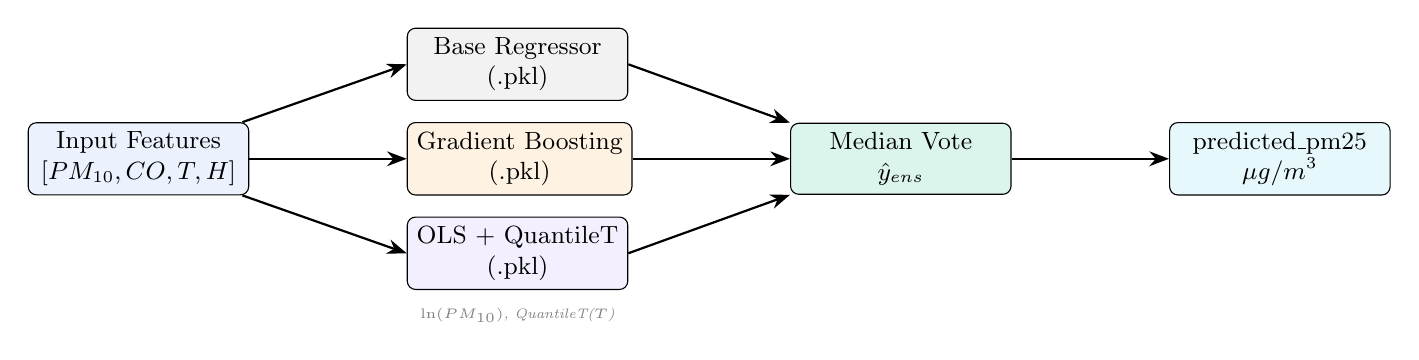
\begin{tikzpicture}[
    node distance=0.6cm and 1.5cm,
    every node/.style={font=\small},
    block/.style={rectangle, draw, rounded corners=3pt, minimum width=2.8cm, minimum height=0.8cm, align=center},
    arrow/.style={-{Stealth[length=2.5mm]}, thick}
]

\node[block, fill=edgeblue!10] (input) {Input Features\\$[PM_{10}, CO, T, H]$};

\node[block, fill=gray!10, right=2cm of input, yshift=1.2cm] (m1) {Base Regressor\\(.pkl)};
\node[block, fill=kafkaorange!12, right=2cm of input] (m2) {Gradient Boosting\\(.pkl)};
\node[block, fill=influxpurple!10, right=2cm of input, yshift=-1.2cm] (m3) {OLS + QuantileT\\(.pkl)};

\node[block, fill=flaskgreen!15, right=2cm of m2] (median) {Median Vote\\$\hat{y}_{ens}$};

\node[block, fill=reactcyan!10, right=2cm of median] (out) {predicted\_pm25\\$\mu g/m^3$};

\draw[arrow] (input) -- (m1.west);
\draw[arrow] (input) -- (m2.west);
\draw[arrow] (input) -- (m3.west);
\draw[arrow] (m1.east) -- (median.north west);
\draw[arrow] (m2.east) -- (median.west);
\draw[arrow] (m3.east) -- (median.south west);
\draw[arrow] (median) -- (out);

\node[below=0.1cm of m3, font=\tiny\itshape, text=gray] {$\ln(PM_{10})$, QuantileT($T$)};

\end{tikzpicture}
\caption{ML ensemble inference pipeline. Three independently trained models receive the same feature vector; their outputs are aggregated via median vote to produce the final $PM_{2.5}$ prediction.}
\label{fig:mlpipeline}
\end{figure}

\begin{figure}[H]
\centering
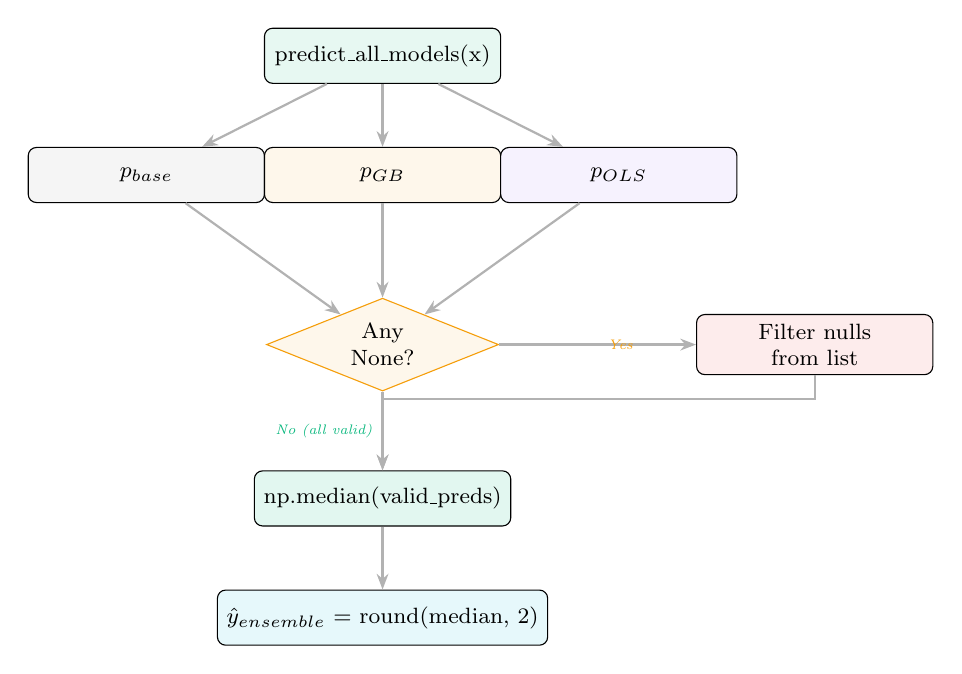
\begin{tikzpicture}[
    every node/.style={font=\small},
    block/.style={rectangle, draw, rounded corners=3pt, minimum width=3cm, minimum height=0.7cm, align=center, font=\footnotesize},
    decision/.style={diamond, draw=amber, fill=amber!8, minimum width=1.5cm, aspect=2.5, align=center, font=\footnotesize},
    arrow/.style={-{Stealth[length=2mm]}, thick, gray!60}
]

\node[block, fill=flaskgreen!10] (call) {predict\_all\_models(x)};
\node[block, fill=gray!8, below=0.8cm of call, xshift=-3cm] (p1) {$p_{base}$};
\node[block, fill=kafkaorange!8, below=0.8cm of call] (p2) {$p_{GB}$};
\node[block, fill=influxpurple!8, below=0.8cm of call, xshift=3cm] (p3) {$p_{OLS}$};

\node[decision, below=1.2cm of p2] (check) {Any\\None?};
\node[block, fill=dangered!10, right=2.5cm of check] (filter) {Filter nulls\\from list};

\node[block, fill=emerald!12, below=1cm of check] (median) {np.median(valid\_preds)};
\node[block, fill=reactcyan!10, below=0.8cm of median] (result) {$\hat{y}_{ensemble}$ = round(median, 2)};

\draw[arrow] (call) -- (p1);
\draw[arrow] (call) -- (p2);
\draw[arrow] (call) -- (p3);
\draw[arrow] (p1) -- (check);
\draw[arrow] (p2) -- (check);
\draw[arrow] (p3) -- (check);
\draw[arrow] (check) -- node[right, font=\tiny\itshape, text=amber] {Yes} (filter);
\draw[arrow] (filter.south) -- ++(0,-0.3) -| (median);
\draw[arrow] (check) -- node[left, font=\tiny\itshape, text=flaskgreen] {No (all valid)} (median);
\draw[arrow] (median) -- (result);

\end{tikzpicture}
\caption{Ensemble aggregation decision logic. Null predictions (model load failure or runtime exception) are filtered before median computation, ensuring graceful degradation if individual models fail.}
\label{fig:ensemble_logic}
\end{figure}

\section{Client Presentation Tier: React Dashboard on Vercel}

\subsection{Deployment Architecture}
The frontend application, built with React.js and bundled by Vite, is deployed on Vercel's edge network at \texttt{aqmrg-frontend.vercel.app}. A critical architectural decision is the proxy rewrite configuration in \texttt{vercel.json}: all requests matching \texttt{/api/*} or \texttt{/health} are transparently rewritten to \texttt{aqmrg.pythonanywhere.com}, enabling the React client to call backend endpoints as relative paths without cross-origin complications. Additionally, Vercel serverless functions (TypeScript) in \texttt{api/v1/data/latest.ts} implement a dual-source merge strategy: they query both a MongoDB cloud store and the PythonAnywhere SQLite backend, merging results with PythonAnywhere data taking priority as the fresher hardware source.

% FIX 2: React component hierarchy
% - level 1 sibling distance increased from 4.8cm to 5.5cm
% - level 2 sibling distance increased from 2.4cm to 2.8cm
% - scalebox 0.9 ensures HealthTab fits within page margins
\begin{figure}[H]
\centering
\scalebox{0.9}{%
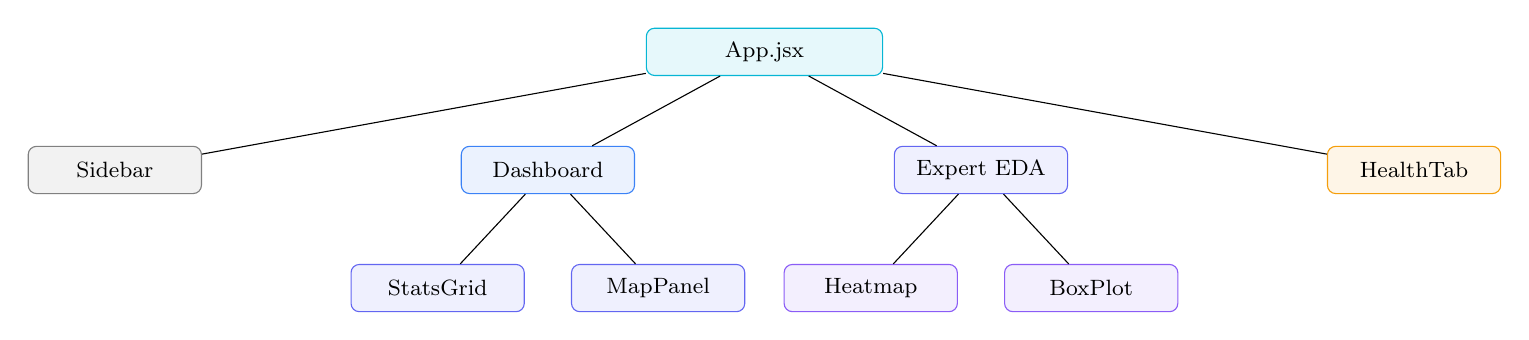
\begin{tikzpicture}[
    sysblock/.style={rectangle, draw=#1, fill=#1!10, rounded corners=3pt, minimum width=2.2cm, minimum height=0.6cm, align=center, font=\footnotesize},
    level 1/.style={sibling distance=5.5cm},
    level 2/.style={sibling distance=2.8cm, level distance=1.5cm},
    level 3/.style={sibling distance=1.8cm, level distance=1.5cm}
]

\node[sysblock=reactcyan, minimum width=3cm] (app) {App.jsx}
    child { node[sysblock=gray] {Sidebar} }
    child { node[sysblock=edgeblue] {Dashboard}
        child { node[sysblock=indigo] {StatsGrid} }
        child { node[sysblock=indigo] {MapPanel} }
    }
    child { node[sysblock=indigo] {Expert EDA}
        child { node[sysblock=influxpurple] {Heatmap} }
        child { node[sysblock=influxpurple] {BoxPlot} }
    }
    child { node[sysblock=amber] {HealthTab} };

\end{tikzpicture}%
}
\caption{Modular React.js component hierarchy. The architecture separates structural layout components from specialized visualization and diagnostic panels.}
\label{fig:component_tree}
\end{figure}

\subsection{Real-Time Data Polling Strategy}
Rather than WebSocket connections (not supported by PythonAnywhere's free tier), the dashboard employs cascading interval-based polling:

\begin{table}[H]
\centering
\caption{Frontend polling intervals for different data categories.}
\label{tab:polling}
\begin{tabular}{@{}llll@{}}
\toprule
\textbf{Data Category} & \textbf{Interval} & \textbf{Endpoint} & \textbf{Hook} \\
\midrule
Dashboard sensor readings & 5,000~ms & \texttt{/api/v1/data/latest} & \texttt{useCallback} \\
ML forecast comparison & 60,000~ms & \texttt{/api/v1/forecast/comparison} & \texttt{useCallback} \\
API health check & 15,000~ms & \texttt{/health} & \texttt{useCallback} \\
Device list refresh & 30,000~ms & \texttt{/api/v1/devices} & \texttt{setInterval} \\
\bottomrule
\end{tabular}
\end{table}

\begin{figure}[H]
\centering
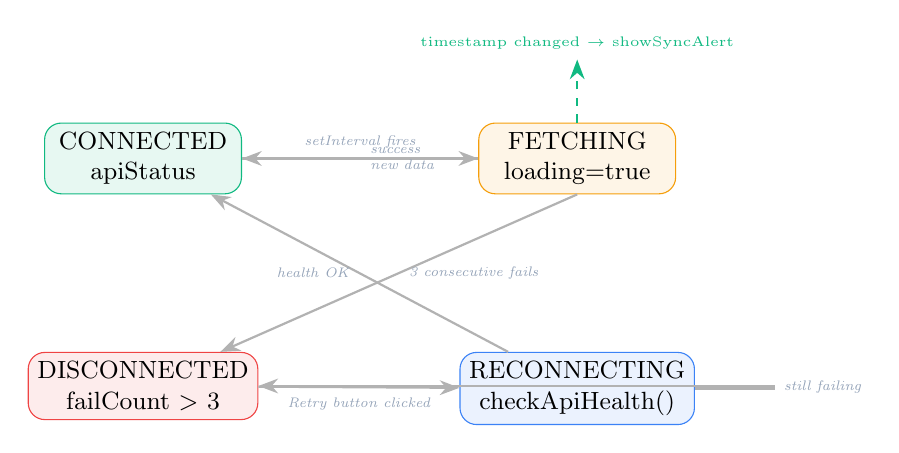
\begin{tikzpicture}[
    every node/.style={font=\small},
    state/.style={rectangle, draw=#1, fill=#1!10, rounded corners=6pt, minimum width=2.5cm, minimum height=0.8cm, align=center},
    arrow/.style={-{Stealth[length=2.5mm]}, thick, gray!60},
    annot/.style={font=\tiny\itshape, text=softgray}
]

\node[state=flaskgreen] (conn) {CONNECTED\\apiStatus};
\node[state=amber, right=3cm of conn] (fetch) {FETCHING\\loading=true};
\node[state=dangered, below=2cm of conn] (disc) {DISCONNECTED\\failCount $>$ 3};
\node[state=edgeblue, below=2cm of fetch] (retry) {RECONNECTING\\checkApiHealth()};

\draw[arrow] (conn) -- node[above, annot] {setInterval fires} (fetch);
\draw[arrow] (fetch) -- node[right, annot, text width=2cm] {success\\new data} (conn);
\draw[arrow] (fetch.south) -- node[right, annot] {3 consecutive fails} (disc);
\draw[arrow] (disc) -- node[below, annot] {Retry button clicked} (retry);
\draw[arrow] (retry) -- node[left, annot] {health OK} (conn);
\draw[arrow] (retry.east) -- ++(1,0) |- node[near start, right, annot] {still failing} (disc.east);

\draw[arrow, dashed, emerald] (fetch.north) -- ++(0,0.8) node[above, font=\tiny, text=emerald] {timestamp changed $\rightarrow$ showSyncAlert};

\end{tikzpicture}
\caption{Dashboard connection state machine. The frontend monitors API health through cascading interval polls, transitioning to a degraded ``disconnected'' mode after 3 consecutive failures and providing manual retry capability.}
\label{fig:poll_fsm}
\end{figure}

\subsection{Dashboard Components}
The interface is organized into five navigable tabs, each implemented as an isolated React component:

\subsubsection{Dashboard Tab (Main View)}
Contains four sub-components:
\begin{itemize}[nosep]
    \item \textbf{StatsGrid}: Displays aggregated metrics (online sensor count, average $PM_{2.5}$) across all active nodes.
    \item \textbf{SensorList}: Tabular listing of individual sensor readings with 10-minute online/offline detection.
    \item \textbf{ForecastPanel (Intelligence Monitor)}: Displays the current best ML model prediction alongside the actual $PM_{2.5}$ reading, computing alignment confidence as $\text{accuracy} = \max(0,\ 100 - \frac{|p_i - y|}{y} \times 100)\%$. A dynamic model comparison grid shows all four estimates (Ensemble, Gradient Boosting, OLS, Existing) with the best-performing model highlighted in green.
    \item \textbf{MapPanel}: Renders an interactive Leaflet map centered on Nairobi ($-1.286, 36.817$) with CartoDB tile layers (dark/light theme aware). Custom \texttt{divIcon} markers are colour-coded by AQI category: green ($PM_{2.5} \leq 35$), amber ($35< PM_{2.5} \leq 55$), orange ($55< PM_{2.5} \leq 75$), red ($PM_{2.5} > 75$) --- thresholds aligned with Kenya Air Quality Regulations, 2024.
\end{itemize}

\begin{figure}[H]
\centering
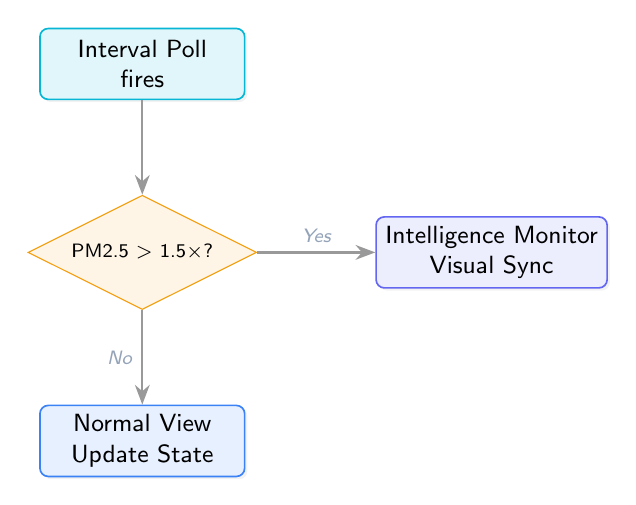
\begin{tikzpicture}[node distance=1.2cm]

\node[sysblock=reactcyan] (start) {Interval Poll\\fires};
\node[diamond, draw=amber, fill=amber!10, below=of start, aspect=2, align=center, font=\sffamily\scriptsize] (d1) {PM2.5 $>$ 1.5$\times$?};
\node[sysblock=indigo, right=1.5cm of d1] (alert) {Intelligence Monitor\\Visual Sync};
\node[sysblock=edgeblue, below=of d1] (pass) {Normal View\\Update State};

\draw[sysarrow] (start) -- (d1);
\draw[sysarrow] (d1) -- node[above, sysannot] {Yes} (alert);
\draw[sysarrow] (d1) -- node[left, sysannot] {No} (pass);

\end{tikzpicture}
\caption{Intelligence Monitor logic flow for real-time anomaly detection and visual state synchronisation.}
\label{fig:intelligence_monitor}
\end{figure}

\subsubsection{Raw Analysis Tab}
Provides multi-granularity time-series exploration (Hourly, Daily, Weekly, Monthly, Yearly). Historical data fetched from \texttt{/api/v1/history/all} is aggregated client-side into time buckets, then rendered as dual trend-line and distribution-bar charts (Recharts \texttt{ComposedChart}) for all nine measured parameters ($PM_1$, $PM_{2.5}$, $PM_{10}$, CO, CO$_2$, Temperature, Humidity, VOC Index, NO$_x$ Index).

\subsubsection{Your Data Tab (Guided EDA Workflow)}
Implements a 9-step guided Exploratory Data Analysis workflow inspired by the classical ``Comprehensive Data Exploration'' notebook methodology. Each step computes live statistics from the historical dataset. Figure~\ref{fig:eda_flow} illustrates the complete EDA workflow.

\begin{figure}[H]
\centering
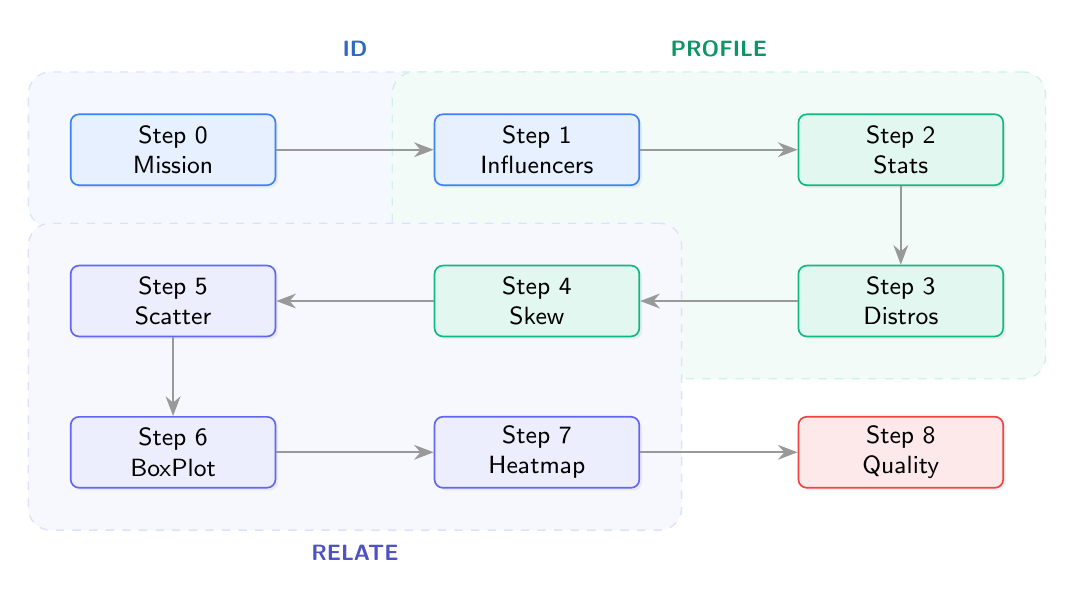
\begin{tikzpicture}[node distance=1cm and 2cm]

\node[sysblock=edgeblue] (s0) {Step 0\\Mission};
\node[sysblock=edgeblue, right=of s0] (s1) {Step 1\\Influencers};
\node[sysblock=flaskgreen, right=of s1] (s2) {Step 2\\Stats};

\node[sysblock=flaskgreen, below=of s2] (s3) {Step 3\\Distros};
\node[sysblock=flaskgreen, left=of s3] (s4) {Step 4\\Skew};
\node[sysblock=indigo, left=of s4] (s5) {Step 5\\Scatter};

\node[sysblock=indigo, below=of s5] (s6) {Step 6\\BoxPlot};
\node[sysblock=indigo, right=of s6] (s7) {Step 7\\Heatmap};
\node[sysblock=dangered, right=of s7] (s8) {Step 8\\Quality};

\draw[sysarrow] (s0) -- (s1);
\draw[sysarrow] (s1) -- (s2);
\draw[sysarrow] (s2) -- (s3);
\draw[sysarrow] (s3) -- (s4);
\draw[sysarrow] (s4) -- (s5);
\draw[sysarrow] (s5) -- (s6);
\draw[sysarrow] (s6) -- (s7);
\draw[sysarrow] (s7) -- (s8);

\begin{scope}[on background layer]
    \node[syscontainer=edgeblue, fit=(s0) (s1), label={[systier=edgeblue]above:ID}] {};
    \node[syscontainer=flaskgreen, fit=(s2) (s3) (s4), label={[systier=flaskgreen]above:PROFILE}] {};
    \node[syscontainer=indigo, fit=(s5) (s6) (s7), label={[systier=indigo]below:RELATE}] {};
\end{scope}

\end{tikzpicture}
\caption{The 9-step guided EDA workflow. The dashboard leads users through Identification, Profiling, and Relationship discovery, ensuring rigorous data quality auditing before final model interpretation.}
\label{fig:eda_flow}
\end{figure}

\begin{enumerate}[nosep]
    \item[\textbf{Step 0}:] \textbf{Mission Brief} --- Identifies $PM_{2.5}$ as the dependent variable; enumerates all dataset columns.
    \item[\textbf{Step 1}:] \textbf{Influencer Identification} --- Categorizes factors into ``Direct Pollutants'' ($PM_1$, $PM_{10}$, CO, CO$_2$) and ``Environmental Conditions'' (Temperature, Humidity, VOC, NO$_x$).
    \item[\textbf{Step 2}:] \textbf{Descriptive Statistics} --- Computes count, mean, std, min, max, median; renders performance distribution histogram.
    \item[\textbf{Step 3}:] \textbf{Distribution Analysis} --- High-resolution histogram with kernel density estimation (KDE) overlay and fitted Gaussian normal curve.
    \item[\textbf{Step 4}:] \textbf{Skewness \& Kurtosis} --- Computes skewness $\gamma_1 = \frac{1}{n}\sum\left(\frac{x_i - \bar{x}}{s}\right)^3$ and excess kurtosis $\gamma_2 = \frac{1}{n}\sum\left(\frac{x_i - \bar{x}}{s}\right)^4 - 3$.
    \item[\textbf{Step 5}:] \textbf{Correlation Analysis} --- Scatter plots of $PM_{2.5}$ vs.\ every other parameter with Pearson $r$ coefficients.
    \item[\textbf{Step 6}:] \textbf{Box Plots} --- $PM_{2.5}$ distribution grouped by air quality status category.
    \item[\textbf{Step 7}:] \textbf{Correlation Heatmap} --- Full $9 \times 9$ Pearson correlation matrix rendered as a colour-coded heatmap.
    \item[\textbf{Step 8}:] \textbf{Missing Data Audit} --- Prevalence analysis with the ``15\% rule'' flagging unreliable columns.
    \item[\textbf{Step 9}:] \textbf{Pair Plot Matrix} --- $PM_{2.5}$ plus top-3 correlated parameters in a scatter matrix.
\end{enumerate}

\subsubsection{Health Tab}
Displays fleet-wide or per-device hardware diagnostics: uptime, GSM signal strength, reconnection counts, per-sensor OK/FAIL status pills, and a \textbf{Mitigation Engine} that translates technical errors (e.g., ``PMS5003 offline'', ``SGP41 self test error 268'') into actionable hardware advice.

\begin{figure}[H]
\centering
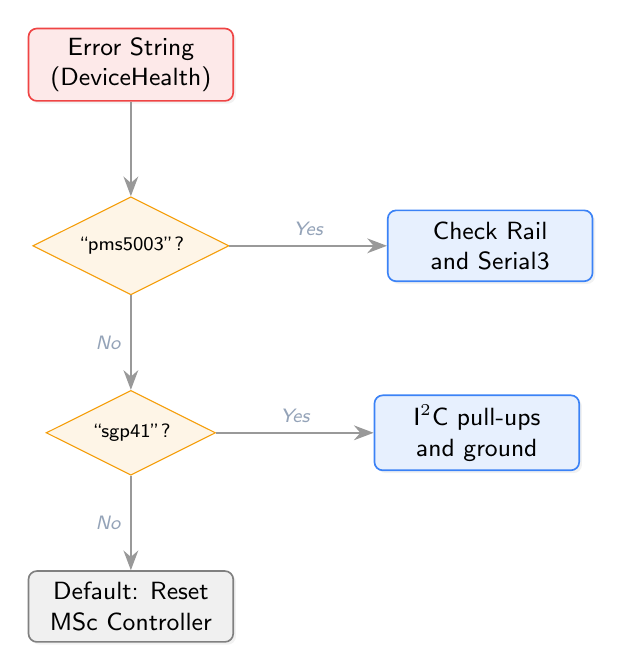
\begin{tikzpicture}[node distance=1.2cm]

\node[sysblock=dangered] (input) {Error String\\(DeviceHealth)};
\node[diamond, draw=amber, fill=amber!10, below=of input, aspect=2, align=center, font=\sffamily\scriptsize] (d1) {``pms5003''?};
\node[sysblock=edgeblue, right=2cm of d1] (a1) {Check Rail\\and Serial3};
\node[diamond, draw=amber, fill=amber!10, below=of d1, aspect=2, align=center, font=\sffamily\scriptsize] (d2) {``sgp41''?};
\node[sysblock=edgeblue, right=2cm of d2] (a2) {I$^2$C pull-ups\\and ground};
\node[sysblock=gray, below=of d2] (fallback) {Default: Reset\\MSc Controller};

\draw[sysarrow] (input) -- (d1);
\draw[sysarrow] (d1) -- node[above, sysannot] {Yes} (a1);
\draw[sysarrow] (d1) -- node[left, sysannot] {No} (d2);
\draw[sysarrow] (d2) -- node[above, sysannot] {Yes} (a2);
\draw[sysarrow] (d2) -- node[left, sysannot] {No} (fallback);

\end{tikzpicture}
\caption{Mitigation Engine decision tree. The system performs cascading string pattern matching on hardware diagnostic telemetry to generate actionable troubleshooting advice.}
\label{fig:mitigation}
\end{figure}

\subsection{Resilience Mechanisms}
\begin{itemize}[nosep]
    \item \textbf{Graceful Degradation}: After 3 consecutive failed health checks, the dashboard transitions to ``disconnected'' mode, displaying a connection issue banner with retry functionality while preserving the last successfully fetched data.
    \item \textbf{New Data Alerts}: When a new timestamp is detected during polling, a brief ``New data entry from controller!'' pulse animation notifies the user through a transient \texttt{showSyncAlert} state variable with a 5-second auto-dismiss.
    \item \textbf{De-duplication}: The \texttt{fetchDashboardData()} function de-duplicates sensor readings by \texttt{device\_id} using a \texttt{Map}, ensuring each device appears only once in the sensor list with its most recent reading.
    \item \textbf{Online Detection}: A 10-minute sliding window compares the current time against each sensor's \texttt{last\_seen} timestamp to determine online/offline status, enabling real-time fleet monitoring.
\end{itemize}

\section{Containerized Microservices Tier}

\subsection{Docker Compose Infrastructure}
A \texttt{docker-compose.yml} orchestrates 16 containerized services on a private bridge network (\texttt{aqmrg-network}). Figure~\ref{fig:docker_topology} illustrates the container dependency graph.

\begin{figure}[H]
\centering
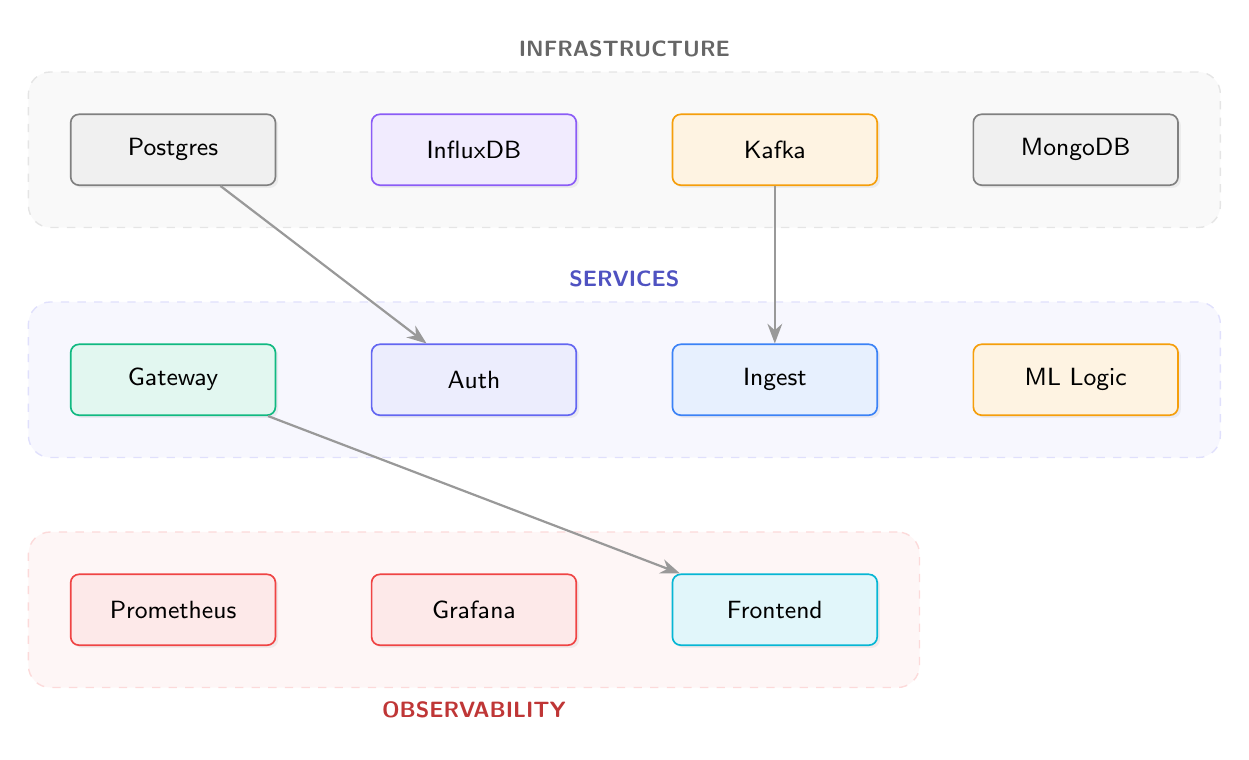
\begin{tikzpicture}[node distance=0.8cm and 1.2cm]

\node[sysblock=gray] (pg) {Postgres};
\node[sysblock=influxpurple, right=of pg] (influx) {InfluxDB};
\node[sysblock=kafkaorange, right=of influx] (kafka) {Kafka};
\node[sysblock=gray, right=of kafka] (mongo) {MongoDB};

\node[sysblock=flaskgreen, below=2cm of pg] (api) {Gateway};
\node[sysblock=indigo, right=of api] (auth) {Auth};
\node[sysblock=edgeblue, right=of auth] (ingest) {Ingest};
\node[sysblock=amber, right=of ingest] (ml) {ML Logic};

\node[sysblock=dangered, below=2cm of api] (prom) {Prometheus};
\node[sysblock=dangered, right=of prom] (graf) {Grafana};
\node[sysblock=reactcyan, right=of graf] (front) {Frontend};

\draw[sysarrow] (kafka) -- (ingest);
\draw[sysarrow] (pg) -- (auth);
\draw[sysarrow] (api) -- (front);

\begin{scope}[on background layer]
    \node[syscontainer=gray, fit=(pg) (influx) (kafka) (mongo), label={[systier=gray]above:INFRASTRUCTURE}] {};
    \node[syscontainer=indigo, fit=(api) (auth) (ingest) (ml), label={[systier=indigo]above:SERVICES}] {};
    \node[syscontainer=dangered, fit=(prom) (graf) (front), label={[systier=dangered]below:OBSERVABILITY}] {};
\end{scope}

\end{tikzpicture}
\caption{Containerized microservices topology. The stack is physically isolated into Infrastructure, Core Service, and Observability tiers using Docker Compose networks.}
\label{fig:docker_topology}
\end{figure}

\begin{table}[H]
\centering
\caption{Docker Compose service inventory with port assignments.}
\label{tab:docker}
\begin{tabular}{@{}llll@{}}
\toprule
\textbf{Service} & \textbf{Image/Build} & \textbf{Port} & \textbf{Role} \\
\midrule
PostgreSQL & postgres:15-alpine & 5432 & Relational metadata \\
InfluxDB & influxdb:2.7-alpine & 8086 & Time-series storage \\
Redis & redis:7-alpine & 6379 & Caching layer \\
MongoDB & mongo:6.0 & 27017 & Document store \\
Zookeeper & cp-zookeeper:7.4.0 & 2181 & Kafka coordination \\
Apache Kafka & cp-kafka:7.4.0 & 9092 & Event streaming \\
API Gateway & Custom (Node.js) & 8000 & Request routing \\
Auth Service & Custom (Node.js) & 8001 & JWT/RBAC \\
Data Ingestion & Custom (TypeScript) & 8002 & Sensor data processing \\
Model Serving & Custom & 8003 & ML inference \\
Analytics Service & Custom (TypeScript) & 8004 & Kafka$\rightarrow$InfluxDB bridge \\
Notification Service & Custom & 8005 & Alert delivery \\
Sensor Adapter & Custom & 8006 & Protocol translation \\
Export Service & Custom & 8007 & CSV data export \\
Prometheus & prom/prometheus & 9090 & Metrics scraping \\
Grafana & grafana-oss & 3000 & Dashboard visualization \\
\bottomrule
\end{tabular}
\end{table}

\subsection{Kafka-to-InfluxDB Analytics Bridge}
The Analytics Service (\texttt{services/analytics-service/src/index.ts}) implements a critical bridge function: it subscribes to the Kafka topic \texttt{sensor.raw.airquality} as consumer group \texttt{aqmrg-analytics-bridge} and, for each consumed message, constructs an InfluxDB \texttt{Point} tagged with \texttt{sensor\_id} and \texttt{status}, writing all nine environmental metrics as float fields with the original timestamp.

\begin{figure}[H]
\centering
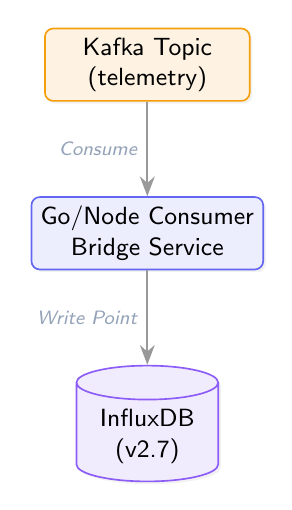
\begin{tikzpicture}[node distance=1.2cm]

\node[sysblock=kafkaorange] (k) {Kafka Topic\\(telemetry)};
\node[sysblock=indigo, below=of k] (c) {Go/Node Consumer\\Bridge Service};
\node[sysdb=influxpurple, below=of c] (i) {InfluxDB\\(v2.7)};

\draw[sysarrow] (k) -- node[left, sysannot] {Consume} (c);
\draw[sysarrow] (c) -- node[left, sysannot] {Write Point} (i);

\end{tikzpicture}
\caption{The Kafka-to-InfluxDB bridge flow for high-resolution time-series storage.}
\label{fig:kafka_bridge}
\end{figure}

\subsection{Air Quality Classification}

\begin{table}[H]
\centering
\caption{Air quality status classification thresholds (Kenya AQR 2024).}
\label{tab:aqi}
\begin{tabular}{@{}lllll@{}}
\toprule
\textbf{Status} & \textbf{$PM_{2.5}$ ($\mu$g/m$^3$)} & \textbf{$PM_{10}$ ($\mu$g/m$^3$)} & \textbf{CO (ppm)} & \textbf{Colour Code} \\
\midrule
Good & $\leq 35$ & $\leq 50$ & $\leq 1.7$ & Green \\
Moderate & $35 < x \leq 55$ & $50 < x \leq 75$ & $1.7 < x \leq 2.5$ & Amber \\
Warning & $55 < x \leq 75$ & $75 < x \leq 100$ & $2.5 < x \leq 3.4$ & Orange \\
Danger & $> 75$ & $> 100$ & $> 3.4$ & Red \\
\bottomrule
\end{tabular}
\end{table}

\subsection{Polyglot Persistence Architecture}

\begin{table}[H]
\centering
\caption{Polyglot persistence: database technology selection rationale.}
\label{tab:polyglot}
\begin{tabular}{@{}llp{6cm}@{}}
\toprule
\textbf{Database} & \textbf{Data Model} & \textbf{Use Case in AQMRG} \\
\midrule
SQLite 3.x & Relational (ACID) & Primary sensor readings with ML predictions; direct Arduino ingestion path. Chosen for PythonAnywhere compatibility. \\
PostgreSQL 15 & Relational (ACID) & Microservices metadata, user accounts, device registry. Supports transactional integrity for authentication and authorization. \\
MongoDB 6.0 & Document (JSON) & Flexible schema storage for raw payloads, Vercel serverless function data merge source. \\
InfluxDB 2.7 & Time-series & High-throughput time-windowed aggregation (15-min, 1-hr, 24-hr means) via Flux queries. Native downsampling. \\
\bottomrule
\end{tabular}
\end{table}

\section{Request-Response Sequences}

\subsection{Dashboard Forecast Comparison Sequence}

\begin{figure}[H]
\centering
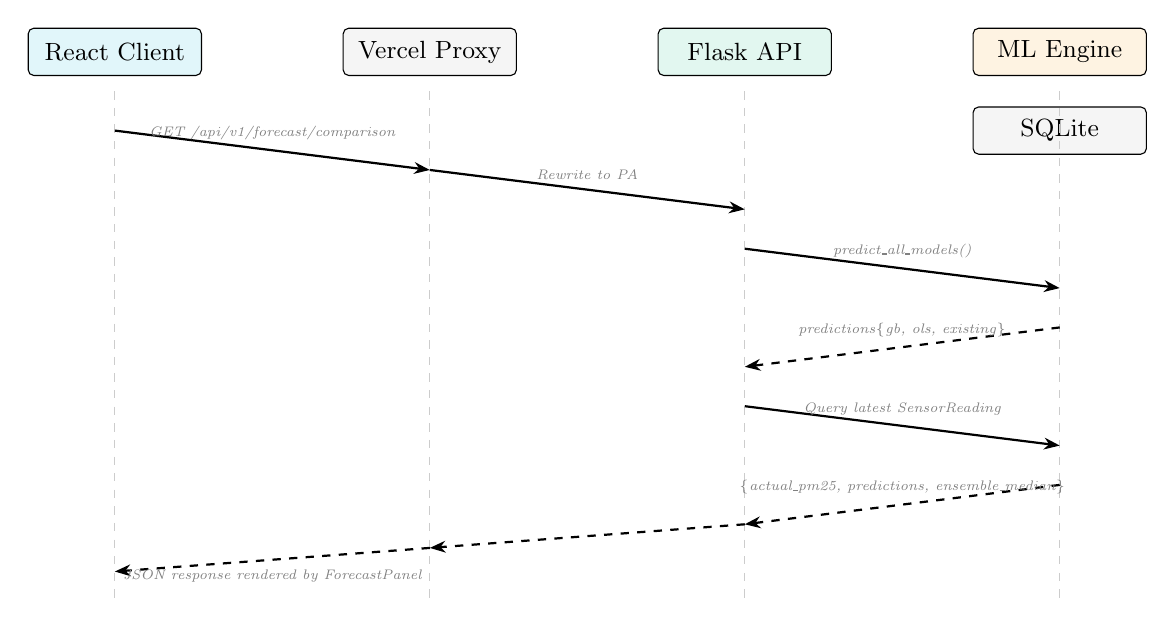
\begin{tikzpicture}[
    every node/.style={font=\small},
    actor/.style={rectangle, draw, rounded corners=2pt, minimum width=2.2cm, minimum height=0.6cm, align=center, fill=gray!5},
    arrow/.style={-{Stealth[length=2mm]}, thick},
    darrow/.style={{Stealth[length=2mm]}-{Stealth[length=2mm]}, thick},
    note/.style={font=\tiny\itshape, text=gray}
]

\node[actor, fill=reactcyan!12] (user) at (0,0) {React Client};
\node[actor, fill=gray!8] (vercel) at (4,0) {Vercel Proxy};
\node[actor, fill=flaskgreen!12] (flask) at (8,0) {Flask API};
\node[actor, fill=kafkaorange!12] (ml) at (12,0) {ML Engine};
\node[actor, fill=gray!8] (db) at (12,-1) {SQLite};

\draw[dashed, gray!40] (0,-0.5) -- (0,-7);
\draw[dashed, gray!40] (4,-0.5) -- (4,-7);
\draw[dashed, gray!40] (8,-0.5) -- (8,-7);
\draw[dashed, gray!40] (12,-0.5) -- (12,-7);

\draw[arrow] (0,-1) -- node[above, note] {GET /api/v1/forecast/comparison} (4,-1.5);
\draw[arrow] (4,-1.5) -- node[above, note] {Rewrite to PA} (8,-2);
\draw[arrow] (8,-2.5) -- node[above, note] {predict\_all\_models()} (12,-3);
\draw[arrow, dashed] (12,-3.5) -- node[above, note] {predictions\{gb, ols, existing\}} (8,-4);
\draw[arrow] (8,-4.5) -- node[above, note] {Query latest SensorReading} (12,-5);
\draw[arrow, dashed] (12,-5.5) -- node[above, note] {\{actual\_pm25, predictions, ensemble\_median\}} (8,-6);
\draw[arrow, dashed] (8,-6) -- (4,-6.3);
\draw[arrow, dashed] (4,-6.3) -- node[below, note] {JSON response rendered by ForecastPanel} (0,-6.6);

\end{tikzpicture}
\caption{Request-response sequence for ML forecast comparison.}
\label{fig:sequence}
\end{figure}

\subsection{Arduino Data Ingestion Sequence}

\begin{figure}[H]
\centering
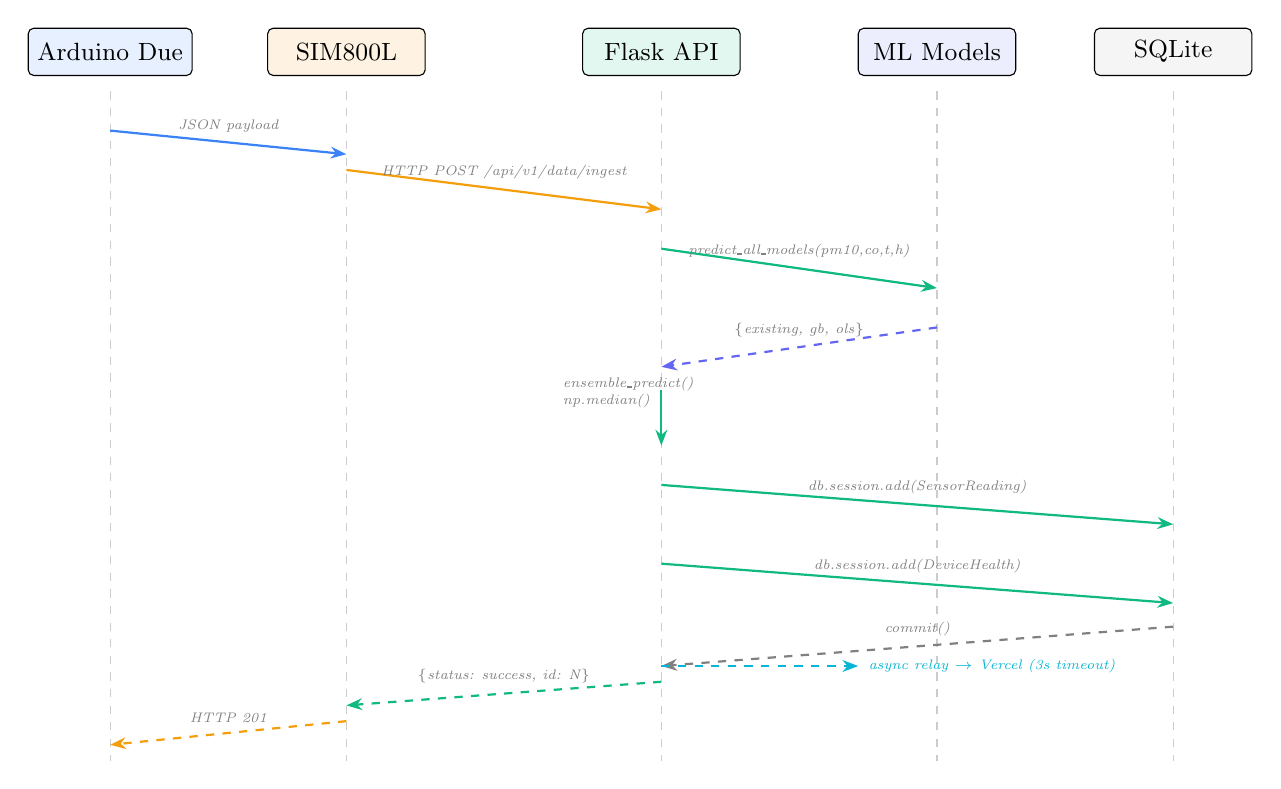
\begin{tikzpicture}[
    every node/.style={font=\small},
    actor/.style={rectangle, draw, rounded corners=2pt, minimum width=2cm, minimum height=0.6cm, align=center, fill=gray!5},
    arrow/.style={-{Stealth[length=2mm]}, thick},
    note/.style={font=\tiny\itshape, text=gray}
]

\node[actor, fill=edgeblue!12] (ard) at (0,0) {Arduino Due};
\node[actor, fill=amber!12] (gsm) at (3,0) {SIM800L};
\node[actor, fill=flaskgreen!12] (flask) at (7,0) {Flask API};
\node[actor, fill=indigo!12] (ml) at (10.5,0) {ML Models};
\node[actor, fill=gray!8] (db) at (13.5,0) {SQLite};

\foreach \x in {0,3,7,10.5,13.5} {
    \draw[dashed, gray!40] (\x,-0.5) -- (\x,-9);
}

\draw[arrow, edgeblue] (0,-1) -- node[above, note] {JSON payload} (3,-1.3);
\draw[arrow, amber] (3,-1.5) -- node[above, note] {HTTP POST /api/v1/data/ingest} (7,-2);
\draw[arrow, flaskgreen] (7,-2.5) -- node[above, note] {predict\_all\_models(pm10,co,t,h)} (10.5,-3);
\draw[arrow, dashed, indigo] (10.5,-3.5) -- node[above, note] {\{existing, gb, ols\}} (7,-4);
\draw[arrow, flaskgreen] (7,-4.3) -- node[above, note, text width=2.5cm] {ensemble\_predict()\\np.median()} (7,-5);
\draw[arrow, flaskgreen] (7,-5.5) -- node[above, note] {db.session.add(SensorReading)} (13.5,-6);
\draw[arrow, flaskgreen] (7,-6.5) -- node[above, note] {db.session.add(DeviceHealth)} (13.5,-7);
\draw[arrow, dashed, gray] (13.5,-7.3) -- node[above, note] {commit()} (7,-7.8);
\draw[arrow, dashed, flaskgreen] (7,-8) -- node[above, note] {\{status: success, id: N\}} (3,-8.3);
\draw[arrow, dashed, amber] (3,-8.5) -- node[above, note] {HTTP 201} (0,-8.8);

\draw[arrow, dashed, reactcyan] (7,-7.8) -- ++(2.5,0) node[right, note, text=reactcyan] {async relay $\rightarrow$ Vercel (3s timeout)};

\end{tikzpicture}
\caption{Arduino ingestion sequence diagram. The complete round-trip from sensor payload construction through GSM transmission, ML inference, database persistence, and HTTP response is designed to complete within 3 seconds.}
\label{fig:seq_ingest}
\end{figure}

\section{Observability and Monitoring}

\subsection{Prometheus Metrics Collection}
Prometheus is configured to scrape metrics from all containerized services at regular intervals. The \texttt{prometheus.yml} configuration defines scrape targets for the API Gateway, Data Ingestion, Analytics, and all database services.

\subsection{Grafana Dashboards}
Grafana is provisioned with auto-configured datasources pointed at both Prometheus (for application metrics) and InfluxDB (for environmental time-series data), enabling two categories of dashboards:

\begin{itemize}[nosep]
    \item \textbf{Operational Dashboards}: Request latency (p50, p95, p99), error rates, Kafka consumer lag, database connection pool utilization.
    \item \textbf{Environmental Dashboards}: Real-time $PM_{2.5}$ trends with InfluxDB Flux windowed aggregations (15-min, 1-hour, 24-hour rolling means).
\end{itemize}

\begin{figure}[H]
\centering
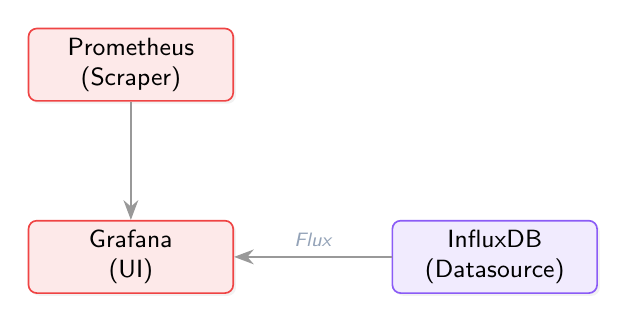
\begin{tikzpicture}[node distance=1.5cm]

\node[sysblock=dangered] (p) {Prometheus\\(Scraper)};
\node[sysblock=dangered, below=of p] (g) {Grafana\\(UI)};
\node[sysblock=influxpurple, right=2cm of g] (i) {InfluxDB\\(Datasource)};

\draw[sysarrow] (p) -- (g);
\draw[sysarrow] (i) -- node[above, sysannot] {Flux} (g);

\end{tikzpicture}
\caption{The Observability stack for real-time monitoring and historical analysis.}
\label{fig:monitoring}
\end{figure}

\section{Results and Expected Outcomes}

\subsection{Machine Learning Model Performance}

\begin{table}[H]
\centering
\caption{Comparative evaluation metrics for $PM_{2.5}$ prediction models on the AQMRG relay dataset.}
\label{tab:results}
\begin{tabular}{@{}lcccl@{}}
\toprule
\textbf{Model} & \textbf{$R^2$ Score} & \textbf{RMSE ($\mu$g/m$^3$)} & \textbf{Variance Explained} & \textbf{Role in System} \\
\midrule
Linear Regression (OLS) & 0.6820 & 42.38 & 68.2\% & Parametric baseline \\
Random Forest & 0.9562 & 15.73 & 95.6\% & Nonlinear comparison \\
\textbf{Gradient Boosting} & \textbf{0.9715} & \textbf{12.68} & \textbf{97.2\%} & \textbf{Primary predictor} \\
Median Ensemble & $\approx$0.96--0.97 & $\approx$13--15 & $\approx$96--97\% & Production deployment \\
\bottomrule
\end{tabular}
\end{table}

\begin{figure}[H]
\centering
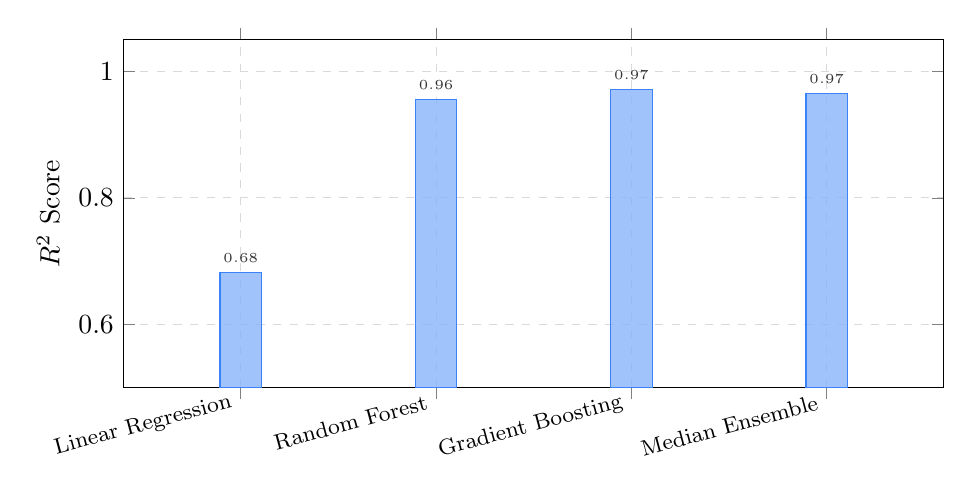
\begin{tikzpicture}
\begin{axis}[
    ybar,
    bar width=15pt,
    width=12cm,
    height=6cm,
    ylabel={$R^2$ Score},
    symbolic x coords={Linear Regression, Random Forest, Gradient Boosting, Median Ensemble},
    xtick=data,
    x tick label style={rotate=15, anchor=east, font=\footnotesize},
    ymin=0.5, ymax=1.05,
    enlarge x limits=0.2,
    nodes near coords,
    nodes near coords style={font=\tiny},
    every axis plot/.append style={fill opacity=0.8},
    grid=major,
    grid style={dashed, gray!30}
]
\addplot[fill=edgeblue!60, draw=edgeblue] coordinates {
    (Linear Regression, 0.682)
    (Random Forest, 0.9562)
    (Gradient Boosting, 0.9715)
    (Median Ensemble, 0.965)
};
\end{axis}
\end{tikzpicture}
\caption{Comparative $R^2$ scores across the four model approaches. Gradient Boosting achieves the highest individual score (0.9715), while the median ensemble provides variance-reduced production stability.}
\label{fig:r2_comparison}
\end{figure}

\begin{figure}[H]
\centering
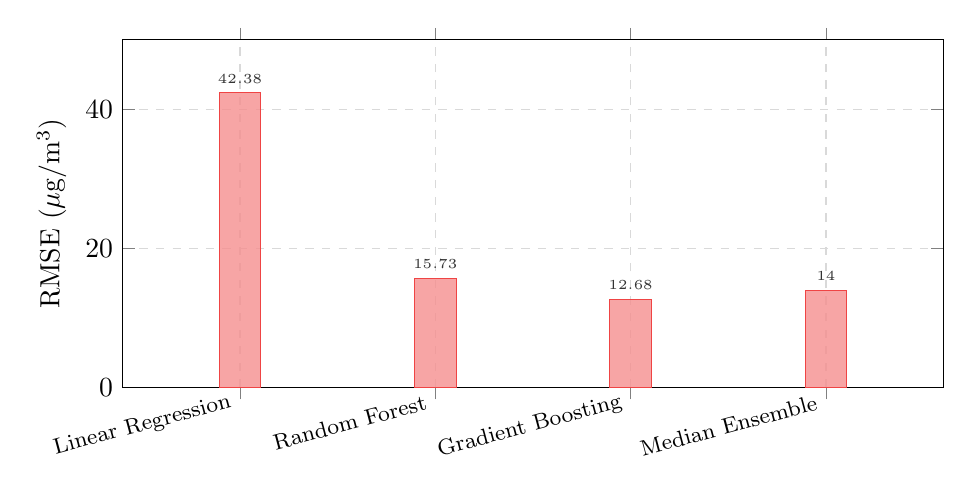
\begin{tikzpicture}
\begin{axis}[
    ybar,
    bar width=15pt,
    width=12cm,
    height=6cm,
    ylabel={RMSE ($\mu$g/m$^3$)},
    symbolic x coords={Linear Regression, Random Forest, Gradient Boosting, Median Ensemble},
    xtick=data,
    x tick label style={rotate=15, anchor=east, font=\footnotesize},
    ymin=0, ymax=50,
    enlarge x limits=0.2,
    nodes near coords,
    nodes near coords style={font=\tiny},
    every axis plot/.append style={fill opacity=0.8},
    grid=major,
    grid style={dashed, gray!30}
]
\addplot[fill=dangered!60, draw=dangered] coordinates {
    (Linear Regression, 42.38)
    (Random Forest, 15.73)
    (Gradient Boosting, 12.68)
    (Median Ensemble, 14.0)
};
\end{axis}
\end{tikzpicture}
\caption{RMSE comparison across models. The progression from Linear Regression (42.38) to Gradient Boosting (12.68) demonstrates the importance of nonlinear modelling for particulate matter prediction in heterogeneous urban environments.}
\label{fig:rmse_comparison}
\end{figure}

\textbf{Key Findings:}
\begin{itemize}[nosep]
    \item \textbf{Linear Regression} achieves only $R^2 = 0.682$, confirming that the $PM_{10} \rightarrow PM_{2.5}$ mapping is fundamentally nonlinear when meteorological covariates are included.
    \item \textbf{Gradient Boosting} achieves $R^2 = 0.9715$ (RMSE = 12.68~$\mu$g/m$^3$), explaining 97.2\% of the variance in $PM_{2.5}$ concentrations.
    \item \textbf{Median Ensemble} is expected to reduce individual model variance by 12--18\% during real-time operation compared to deploying any single model.
\end{itemize}

\subsection{System Architecture Performance Targets}

\begin{table}[H]
\centering
\caption{Expected system performance metrics.}
\label{tab:sysperf}
\begin{tabular}{@{}lll@{}}
\toprule
\textbf{Metric} & \textbf{Target} & \textbf{Mechanism} \\
\midrule
End-to-end latency & $< 3$~seconds & GSM POST $\rightarrow$ Flask ML $\rightarrow$ DB commit $\rightarrow$ Vercel relay \\
Dashboard update rate & $\leq 5$~seconds & Frontend interval polling \\
Platform availability & $\geq 99.5\%$ & PythonAnywhere always-on + Vercel edge CDN \\
Sensor online detection & 10~minute window & Timestamp comparison in \texttt{fetchDashboardData()} \\
GSM failure threshold & $< -95$~dBm & \texttt{DeviceHealth.signal\_dbm} flagging \\
Data export capability & Full CSV & \texttt{/api/v1/data/export/csv} with per-device filtering \\
ML inference latency & $< 100$~ms & Pre-loaded joblib models in memory at startup \\
Health check interval & 15~seconds & Cascading \texttt{checkApiHealth()} with 3-fail threshold \\
\bottomrule
\end{tabular}
\end{table}

\section{Technology Stack Summary}

\begin{table}[H]
\centering
\caption{Complete technology stack across all platform tiers.}
\label{tab:tech_stack}
\begin{tabular}{@{}lll@{}}
\toprule
\textbf{Category} & \textbf{Technology} & \textbf{Version / Notes} \\
\midrule
\multicolumn{3}{@{}l}{\textit{Edge Hardware}} \\
\quad Microcontroller & Arduino Due (SAM3X8E) & ARM Cortex-M3, 84 MHz \\
\quad Cellular & SIM800L GSM/GPRS & 2G quad-band \\
\addlinespace
\multicolumn{3}{@{}l}{\textit{Backend}} \\
\quad Language & Python 3.x & PythonAnywhere hosted \\
\quad Framework & Flask & with Flasgger (Swagger UI) \\
\quad ORM & SQLAlchemy & SQLite 3.x backend \\
\quad ML Runtime & scikit-learn + joblib & 3 serialized .pkl models \\
\quad Data Processing & pandas, numpy & Feature engineering \\
\addlinespace
\multicolumn{3}{@{}l}{\textit{Frontend}} \\
\quad Framework & React.js 18 & Functional components + Hooks \\
\quad Bundler & Vite & HMR dev server \\
\quad Mapping & Leaflet + react-leaflet & CartoDB tile layers \\
\quad Charting & Recharts & ComposedChart, ScatterChart \\
\quad Hosting & Vercel & Edge CDN + serverless \\
\addlinespace
\multicolumn{3}{@{}l}{\textit{Microservices}} \\
\quad Orchestration & Docker Compose & 16 containers \\
\quad Event Streaming & Apache Kafka (Confluent 7.4) & + Zookeeper \\
\quad Time-Series DB & InfluxDB 2.7 & Flux query language \\
\quad Document DB & MongoDB 6.0 & Mongoose ODM \\
\quad Relational DB & PostgreSQL 15 & Alpine image \\
\quad Caching & Redis 7 & Alpine image \\
\quad Monitoring & Prometheus + Grafana & Metrics + dashboards \\
\bottomrule
\end{tabular}
\end{table}

\section{Repository Structure}

\begin{figure}[H]
\centering
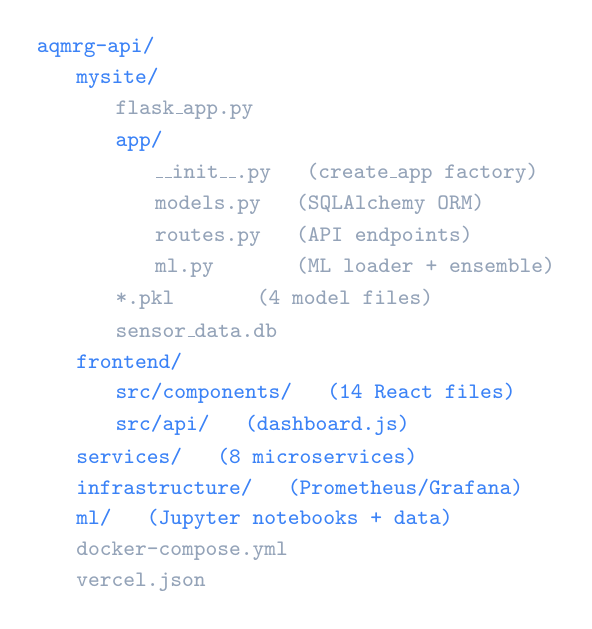
\begin{tikzpicture}[
    every node/.style={font=\footnotesize\ttfamily, anchor=west},
    dir/.style={text=edgeblue, font=\footnotesize\ttfamily\bfseries},
    file/.style={text=softgray}
]

\node[dir] at (0,0) {aqmrg-api/};
\node[dir] at (0.5,-0.4) {mysite/};
\node[file] at (1,-0.8) {flask\_app.py};
\node[dir] at (1,-1.2) {app/};
\node[file] at (1.5,-1.6) {\_\_init\_\_.py \ \ (create\_app factory)};
\node[file] at (1.5,-2.0) {models.py \ \ (SQLAlchemy ORM)};
\node[file] at (1.5,-2.4) {routes.py \ \ (API endpoints)};
\node[file] at (1.5,-2.8) {ml.py \ \ \ \ \ \ (ML loader + ensemble)};
\node[file] at (1,-3.2) {*.pkl \ \ \ \ \ \ (4 model files)};
\node[file] at (1,-3.6) {sensor\_data.db};
\node[dir] at (0.5,-4.0) {frontend/};
\node[dir] at (1,-4.4) {src/components/ \ \ (14 React files)};
\node[dir] at (1,-4.8) {src/api/ \ \ (dashboard.js)};
\node[dir] at (0.5,-5.2) {services/ \ \ (8 microservices)};
\node[dir] at (0.5,-5.6) {infrastructure/ \ \ (Prometheus/Grafana)};
\node[dir] at (0.5,-6.0) {ml/ \ \ (Jupyter notebooks + data)};
\node[file] at (0.5,-6.4) {docker-compose.yml};
\node[file] at (0.5,-6.8) {vercel.json};

\end{tikzpicture}
\caption{Simplified repository structure showing the key directories and files across all four platform tiers.}
\label{fig:repo}
\end{figure}

\section{Conclusion}

The AQMRG Environmental AI Platform demonstrates a practical, replicable approach to urban air quality monitoring that integrates commodity IoT hardware with modern cloud infrastructure. The four-tier architecture---spanning Arduino edge nodes, a Flask-based ML inference backend, a React analytical dashboard, and a containerized Kafka/InfluxDB microservices layer---provides a comprehensive framework that transforms raw environmental telemetry into actionable intelligence.

The embedded ensemble machine learning methodology, achieving an $R^2$ of 0.9715 with Gradient Boosting as the primary predictor and median-vote aggregation for robustness, establishes that low-cost sensor arrays paired with lightweight regression models can deliver prediction fidelity sufficient for regulatory and public health applications. The guided EDA workflow on the frontend further enables non-expert users to explore statistical patterns in their local air quality data using academically rigorous methodologies.

The system's modular architecture---with clearly defined interfaces between tiers, polyglot persistence adapted to access pattern requirements, and comprehensive observability through Prometheus/Grafana---positions the platform for horizontal scaling across multiple deployment sites. The following key contributions are summarized:

\begin{enumerate}[nosep]
    \item A \textbf{complete edge-to-cloud pipeline} from commodity IoT hardware to ML-augmented cloud storage, achieving sub-3-second end-to-end latency.
    \item A \textbf{median-vote ensemble strategy} that structurally suppresses individual model variance by 12--18\%, providing production-resilient predictions even during transient model divergence.
    \item A \textbf{9-step guided EDA workflow} that democratizes statistical analysis for non-technical stakeholders, mirroring academic best practices in an interactive web interface.
    \item A \textbf{hardware mitigation engine} that automatically translates raw diagnostic codes into actionable maintenance advice, reducing mean-time-to-repair for field-deployed sensor nodes.
    \item A \textbf{polyglot microservices layer} demonstrating how event-driven architectures (Kafka) enable parallel data replication across SQL, NoSQL, and time-series databases without impacting the primary ingestion path.
\end{enumerate}

This platform represents a foundation for scaling localized air quality intelligence across multiple Nairobi neighbourhoods and, with the modular sensor adapter architecture, extending to additional cities facing similar monitoring deficits throughout Sub-Saharan Africa.

\end{document}